% ===========================================================================
% EC8203 Applied Big Data Engineering - Mini Project Report
% Ride-Hailing Fleet Operations: a Lambda architecture data platform
%
% Build:  latexmk -pdf main.tex     (or: pdflatex main.tex, twice)
% Figures: docs/report/figures/  - diagrams are vector PDFs built by
%          `make diagrams`; screenshots are PNGs captured by `make figures`.
% ===========================================================================
\documentclass[11pt,a4paper]{article}

\usepackage[margin=2.2cm]{geometry}
\usepackage{amsmath}
\usepackage{graphicx}
\usepackage{booktabs}
\usepackage{tabularx}
\usepackage{longtable}
\usepackage{float}
\usepackage{setspace}
\usepackage{titlesec}
\usepackage{xcolor}
\usepackage{caption}
\usepackage{enumitem}
\usepackage[T1]{fontenc}
\usepackage{lmodern}
\usepackage{microtype}
\usepackage[hidelinks,colorlinks=true,linkcolor=linknavy,citecolor=linknavy,
            urlcolor=linknavy]{hyperref}

\definecolor{linknavy}{HTML}{16447A}
\definecolor{rulegrey}{HTML}{5A6672}
\definecolor{callbg}{HTML}{F4F6F8}

\setstretch{1.0}
\setlist{nosep,leftmargin=1.4em}
\titleformat{\section}{\large\bfseries}{\thesection.}{0.6em}{}
\titleformat{\subsection}{\normalsize\bfseries}{\thesubsection.}{0.6em}{}
\titlespacing*{\section}{0pt}{12pt}{5pt}
\titlespacing*{\subsection}{0pt}{9pt}{3pt}
\captionsetup{font=small,labelfont=bf,skip=3pt}
\setlength{\textfloatsep}{8pt}\setlength{\intextsep}{8pt}
\renewcommand{\arraystretch}{1.15}

% A call-out box, used for the simulated-clock declaration the brief demands
% be stated clearly.
\newcommand{\callout}[2]{%
  \begin{center}\fcolorbox{rulegrey}{callbg}{%
    \begin{minipage}{0.95\linewidth}\small\textbf{#1}\\[2pt]#2\end{minipage}}\end{center}}

% ---------------------------------------------------------------------------
% FILL THESE IN. Collected here so the cover page needs editing in one place.
% ---------------------------------------------------------------------------
\newcommand{\authorA}{Jathur}          \newcommand{\indexA}{EG/20XX/XXXX}
\newcommand{\authorB}{Shamil}          \newcommand{\indexB}{EG/20XX/XXXX}
\newcommand{\authorC}{Rifath}          \newcommand{\indexC}{EG/20XX/XXXX}
\newcommand{\groupnumber}{Group XX}
\newcommand{\submissiondate}{\today}
\newcommand{\repourl}{https://github.com/jathurT/ride-hailing-lambda}
% ---------------------------------------------------------------------------

\begin{document}

% ------------------------------- cover page -------------------------------
\begin{titlepage}
    \centering
    
\includegraphics[width=3cm]{Logo.jpeg}\par\vspace{0.9cm}
    {\LARGE \textbf{Department of Electrical and Information Engineering}}\\[0.4cm]
    {\Large \textbf{University of Ruhuna}}\\[1.4cm]
    {\Large \textbf{Mini Project Report}}\\[0.3cm]
    {\large \textbf{Applied Big Data Engineering}}\\[0.2cm]
    {\large \textbf{EC8203}}\\[1.0cm]

    {\large\itshape Ride-Hailing Fleet Operations:}\\[0.2cm]
    {\large\itshape a Lambda Architecture Data Platform}\\[2.4cm]

    \begin{tabular}{ll}
      \large \textbf{\authorA} & \large \indexA \\[0.25cm]
      \large \textbf{\authorB} & \large \indexB \\[0.25cm]
      \large \textbf{\authorC} & \large \indexC \\
    \end{tabular}\\[1.0cm]

    {\large \textbf{Computer Engineering (CE)}}\\[0.3cm]
    {\large \textbf{\groupnumber}}\\[1.6cm]
    {\large \submissiondate}\\[0.8cm]
    {\small Source code: \url{\repourl}}
\end{titlepage}

\clearpage
\phantomsection
\addcontentsline{toc}{section}{Contents}
\tableofcontents
\clearpage

% ===========================================================================
\section{Introduction and Use Case}

A ride-hailing operator runs a fleet of vehicles that emit telemetry continuously,
and settles running costs against invoices that fuel and garage partners submit once
a day. Dispatch staff need to see the fleet as it is now. Finance needs to know which
vehicles are losing money once those costs are applied. This project implements the
data platform that answers both, from the same data.

The assignment poses the question directly:

\callout{Business question (Use Case 1)}{%
\emph{``What is fleet utilization and earnings by area/time-of-day \textbf{right now},
and which vehicles are \textbf{becoming unprofitable} once \textbf{yesterday's}
fuel/maintenance costs are factored in?''}}

That single sentence contains two questions, and separating them is the whole of the
architectural argument that follows.

\textbf{Question A --- ``right now''} is asked by dispatch operations, continuously,
on a wall-mounted dashboard. Its latency budget is seconds. Its accuracy tolerance is
loose: a utilization figure of 71\,\% rather than 72\,\% changes no decision anybody
makes.

\textbf{Question B --- ``becoming unprofitable, given yesterday's costs''} is asked by
finance, once a day. Its latency budget is hours, and not by concession: the partner
expense file \emph{does not exist} until the day has ended, so no architecture can
answer it sooner. Its accuracy tolerance is zero, because the figure feeds driver
settlements. And the word \textbf{becoming} makes it a question about a trajectory
rather than a balance, which means it needs history.

One question forgives error and demands speed. The other forgives delay and demands
correctness. Any architecture that forces both down a single processing path must
compromise one of them --- and Section~\ref{sec:arch} argues that this, rather than
any property of the technologies involved, is why the system is built as a Lambda
architecture.

\subsection{Stakeholders and system boundary}

Figure~\ref{fig:d1} shows what crosses the system boundary and who depends on it. It
deliberately names no technology: a reader who knows nothing about Kafka should still
be able to see what the platform is for.

\begin{figure}[H]\centering
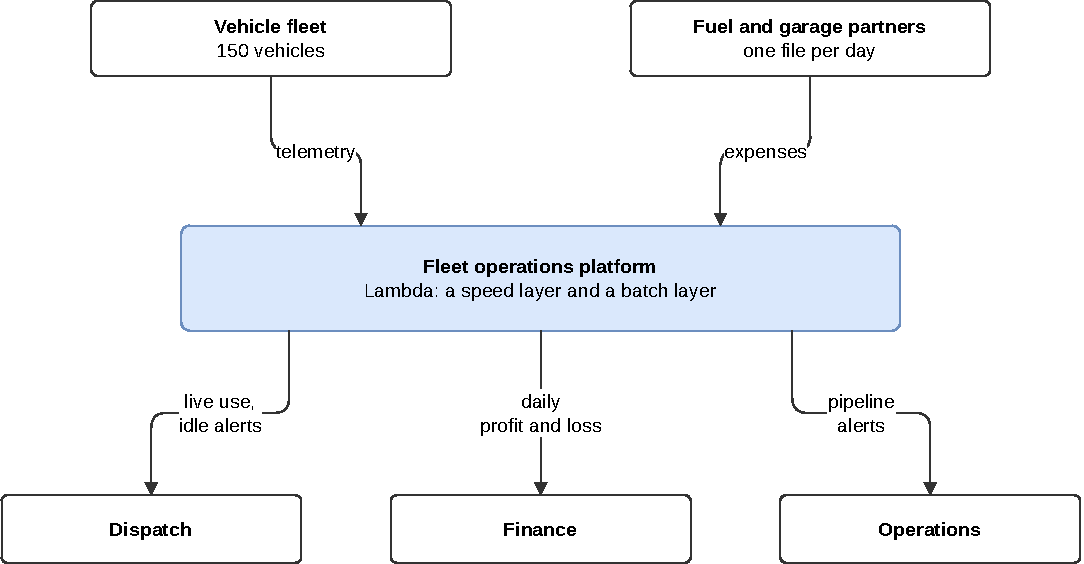
\includegraphics[width=0.84\linewidth]{figures/D1-context.pdf}
\caption{System context. The two sources differ in shape --- one continuous, one a
daily file --- and the two consumers differ in what they will trade away. That
tension is the reason the architecture has two paths.}
\label{fig:d1}
\end{figure}

% ===========================================================================
\section{Business Requirements Interpretation}

The business question was decomposed into functional and non-functional requirements
before any technology was chosen. The non-functional targets are stated as numbers so
that Section~\ref{sec:results} can report whether they were met rather than asserting
that they were.

\begin{table}[H]\centering\small
\begin{tabularx}{\linewidth}{@{}llXl@{}}
\toprule
\textbf{ID} & \textbf{Requirement} & \textbf{Satisfied by} & \textbf{Target} \\
\midrule
FR-1 & Live fleet utilization by zone & Speed layer $\rightarrow$ \texttt{/api/v1/fleet/live} & --- \\
FR-2 & Earnings by area and time of day & \texttt{fact\_zone\_hourly} (exact) + Redis (live) & --- \\
FR-3 & Per-vehicle daily profitability vs.\ expenses & Batch layer $\rightarrow$ \texttt{fact\_vehicle\_daily\_pnl} & --- \\
FR-4 & Identify vehicles \emph{becoming} unprofitable & 7-day rolling average + trend slope & 7 sim-days \\
FR-5 & Threshold alert on prolonged idling & Stateful streaming detector & $\geq$45 sim-min \\
FR-6 & Consolidated daily view & Provisioned Grafana dashboards & 1 / sim-day \\
\midrule
NFR-1 & Live-view freshness & Micro-batch trigger, 10\,s & $<$30\,s real \\
NFR-2 & Profitability accuracy & Exact recompute over master dataset & exact \\
NFR-3 & Restatement handling & Upsert on \texttt{(vehicle\_id, sim\_date)} & idempotent \\
NFR-4 & Pipeline failure detection & Prometheus alert rules & $<$3\,min \\
NFR-5 & Reproducibility & Docker Compose & 1 command \\
\bottomrule
\end{tabularx}
\caption{Requirements, and where each is discharged.}
\end{table}

\callout{Simulated clock --- stated explicitly, as the brief requires}{%
One simulated day is compressed into \textbf{300 real seconds}
(\texttt{SIM\_DAY\_SECONDS=300}), a speed-up of \textbf{288$\times$}. The simulation
begins at simulated date 2026-03-01. Every container derives simulated time from one
shared anchor file written once at start-up, so no two services can disagree about
what day it is. Throughout this report, durations are marked \emph{real} or
\emph{simulated}; where a figure could be read either way it is given in both. A
30-simulated-minute watermark, for instance, is 6.25 real seconds.}

% ===========================================================================
\section{Architecture Decision: Lambda versus Kappa}
\label{sec:arch}

The decision was made against the eight criteria the module itself sets out, used
here as sub-headings so that the reasoning can be followed criterion by criterion
rather than taken on trust. Two of the eight favour Kappa; both are conceded openly
in \S\ref{sec:concede} and mitigated in code rather than argued away.

\subsection{Latency requirements}

The criterion assumes one application with one latency budget. This application has
two, simultaneously. Lambda's defining property is that it provides a low-latency
path \emph{and} a high-latency path from the same source, which is precisely the
shape of the requirement.

The point worth emphasising is that the batch layer's latency is \textbf{not a
limitation we accepted}. It is a property of the business process being modelled:
partners submit costs at the end of the day, so a T+1 file cannot be available at T.
\textbf{Favours Lambda.}

\subsection{Data volume}

At demo scale, 150 vehicles emitting every 3 simulated minutes produce
\textbf{72{,}000 events per simulated day} ($\approx$240\,events/s). At a realistic
operator scale --- 5{,}000 vehicles on a 30-second real interval --- that is
\textbf{14.4 million events per day}. Answering whether a vehicle is \emph{becoming}
unprofitable needs a trailing window of 7--30 days, so 100--430 million events must
be queryable at rest.

That is unambiguously the module's first named workload type, \emph{``batch
processing of big data sources at rest''}. Notably, the same criterion pushes the
sibling use case (hospital ward vitals, $\approx$3{,}840 events/simulated day,
roughly 19$\times$ smaller) toward Kappa --- the criterion is doing real
discriminating work here, not being cited decoratively. \textbf{Favours Lambda.}

\subsection{Historical data analysis --- decisive}

The word \textbf{becoming} carries the weight. The operator is not asking which
vehicles lost money yesterday, which is a one-day lookup. They are asking which are
on a deteriorating trajectory, which requires comparing each vehicle's cost/revenue
position across a trailing window and detecting a trend. The implementation computes
a 7-simulated-day rolling net profit and a least-squares slope, and classifies each
vehicle \texttt{HEALTHY}, \texttt{WATCH} or \texttt{UNPROFITABLE}.

Serving that from stream state would mean either holding weeks of state inside the
streaming job --- expensive, fragile, and lost on restart --- or retaining weeks in
Kafka and replaying. Both reintroduce, in a worse form, exactly the batch processing
Kappa claims to remove. \textbf{Favours Lambda, decisively.}

\subsection{Data reprocessing --- decisive}

This is the strongest technical argument, and it is not hypothetical: it is how fuel
and garage invoicing actually works. \textbf{A partner submits a corrected expense
file for a previous day} --- a fuel card mis-assigned, a maintenance charge billed to
the wrong vehicle, a rebate applied late.

\begin{itemize}
\item \textbf{Under Lambda:} the corrected file lands, Airflow re-triggers the DAG for
that simulated date, Spark re-reads \emph{that one Parquet partition}, re-joins, and
upserts on \texttt{(vehicle\_id, sim\_date)}. Cost is one partition scan. The
operation is idempotent --- \S\ref{sec:results} shows a re-run changing nothing.
\item \textbf{Under Kappa:} the same correction requires replaying every telemetry
event for that day to recompute the join. At realistic scale that is 14.4 million
events reprocessed to fix a handful of expense rows.
\end{itemize}

The cost of a correction should be proportional to the correction, not to the largest
dataset in the system. \textbf{Favours Lambda, decisively.}

\subsection{Fault tolerance}

If the streaming job crashes and loses in-flight state, the live dashboard is stale
until it restarts --- an availability problem. The financial record is untouched,
because it is derived from immutable Parquet by a job that can be re-run to the
identical answer. The speed layer is \emph{disposable by design}: Redis can be
flushed and nothing permanent is lost. This was demonstrated accidentally during
development, when Redis was restarted and the speed view rebuilt itself within
seconds while the batch figures were entirely unaffected.

Under Kappa the streaming job's state \emph{is} the record of truth, so corrupting it
is a data-integrity incident rather than an availability one. Lambda gives a
\textbf{system of record} (Parquet + PostgreSQL) that is independent of the
\textbf{system of engagement} (Redis). \textbf{Favours Lambda.}

\subsection{Accuracy}

The module describes Lambda as offering \emph{``immediate but less accurate''}
results alongside \emph{``high accuracy''}. That is not a compromise to work around
here --- it is a precise description of what the business question asks for. Question~A
wants immediate and tolerates approximate; Question~B wants exact and tolerates delay.
Lambda was chosen \emph{because} the business has that split, not in spite of it.

The speed layer is knowingly approximate in three documented ways: distinct counts
are HyperLogLog ($\approx$2\,\% error); events later than the 30-simulated-minute
watermark are dropped from windowed aggregates (they still reach the master dataset,
so the batch layer sees them); and the newest sliding window is only partially
filled. The batch layer reconciles all three. Every API response states which of the
two produced each row. \textbf{Favours Lambda.}

\subsection{Complexity and cost --- the two we concede}
\label{sec:concede}

\textbf{Complexity favours Kappa, and we concede it.} The module names two specific
Lambda drawbacks and this project has both. What was done about them:

\emph{On ``managing multiple codebases''} --- there is exactly \textbf{one}. All
business logic lives in \texttt{src/fleet/transforms/}, pure DataFrame-in,
DataFrame-out functions containing no streaming or batch concepts. The speed-layer
entry point calls them inside \texttt{foreachBatch}; the batch-layer entry point
calls \emph{the same functions} on a static DataFrame. They are unit-tested once. An
architecture test enforces that neither layer defines transformation logic of its
own. The criticism reduces to ``two entry points over one tested library'', which is
a demonstrable reduction rather than a rhetorical one.

\emph{On ``reconciling data between systems''} --- the two views are not hoped to
agree; a boundary is defined and enforced. Section~\ref{sec:merge} describes it, and
Section~\ref{sec:results} shows it holding on live data.

\textbf{Cost favours Kappa on components, and we contest it on storage.} Lambda here
runs more containers, which is real. But the master dataset is columnar Parquet on
object storage --- the cheapest durable tier --- while Redis holds only the current
window under a 2-simulated-hour TTL, keeping the expensive tier tiny. Kafka retention
is therefore only 7 days, because under Lambda the log does not have to be the
historical store. A Kappa system wanting 30 days of replayable history must pay for
30 days of \emph{broker-attached} storage, which is far more expensive per byte. The
module's cost criterion penalises Lambda for extra storage; for this workload it is
plausibly Kappa that would pay more. \textbf{Conceded on components; contested on
storage.}

\subsection{Summary}

\begin{table}[H]\centering\small
\begin{tabularx}{\linewidth}{@{}clcX@{}}
\toprule
\textbf{\#} & \textbf{Criterion} & \textbf{Favours} & \textbf{Note} \\
\midrule
1 & Latency requirements & Lambda & Two latencies at once; batch latency is inherent to the source \\
2 & Data volume & Lambda & 14.4\,M events/day at scale; 7--30 day window at rest \\
3 & Complexity & \emph{Kappa} & \textbf{Conceded}; mitigated by shared \texttt{transforms/} and an explicit merge boundary \\
4 & Historical data analysis & \textbf{Lambda} & \textbf{Decisive} --- ``\emph{becoming}'' is a multi-day trend \\
5 & Cost & \emph{Kappa} & \textbf{Conceded} on components; contested on storage \\
6 & Fault tolerance & Lambda & Financial record independent of streaming state \\
7 & Data reprocessing & \textbf{Lambda} & \textbf{Decisive} --- partition re-run vs.\ full-day replay \\
8 & Accuracy & Lambda & The question itself has a split accuracy requirement \\
\bottomrule
\end{tabularx}
\caption{Six of eight criteria favour Lambda, including both decisive ones. The two
that favour Kappa are conceded rather than argued away.}
\end{table}

\subsection{The rejected alternative: Kappa}

A rejection is only credible if the case for the rejected option is made properly
first, so it is made here before it is answered.

\textbf{The honest case for Kappa.} One processing path, one codebase, one set of
semantics --- and therefore nothing for the two views to disagree about, which is
Lambda's headline weakness eliminated rather than mitigated. Fewer containers, no
object store, no high-water-mark bookkeeping. Lower infrastructure cost in the
module's terms. And --- the strongest point --- \textbf{the expense file could
genuinely be modelled as a stream}: publish each row to a log-compacted
\texttt{fleet.expenses} topic keyed by \texttt{(vehicle\_id, sim\_date)}, so that a
restatement is simply a later record under the same key and compaction keeps the
newest. A stream--stream join with a long watermark would then yield profitability
continuously rather than daily. This is a legitimate design, and at demo volume
(72\,k events/simulated day) replay would be cheap.

\textbf{Why it lost.} Four reasons, in order of weight:

\begin{enumerate}
\item \emph{The historical requirement is not incidental --- it is the question.}
Kappa's own weakness, in the module's words, is that it \emph{``may not be as
suitable for historical data analysis''}, and historical analysis is what
``becoming'' demands.
\item \emph{Reprocessing cost points the wrong way.} Correcting a few expense rows
should not cost a full day's telemetry replay, and this is a recurring operational
cost, not a one-off.
\item \emph{The auditability story is weaker.} Per-vehicle profitability feeds driver
settlements. ``Here is the immutable, addressable partition for 2026-03-14 and the
deterministic job that produced this figure from it'' is a materially better answer to
an auditor than ``we replayed the log and this is what came out''.
\item \emph{It forces an awkward modelling of a genuinely batch source.} A CSV a
garage uploads once a day is not an event stream. Publishing it to Kafka to satisfy an
architectural rule adds a producer, a topic, a serialization contract and a compaction
policy, and buys nothing an object-store landing zone does not already give. Choosing
an architecture that makes a natural batch source awkward is a signal the architecture
is wrong for the problem.
\end{enumerate}

\textbf{What would change our minds.} We would switch to Kappa if all three of the
following held: the profitability question became continuous rather than daily (costs
streamed from telematics fuel sensors rather than invoiced nightly); \emph{and} the
historical window shrank to something a streaming job can hold in state --- hours, not
weeks; \emph{and} auditability of the financial figure ceased to be a requirement.
Absent all three, Lambda is the right call for this use case.

% ===========================================================================
\section{Architecture Design}

\begin{figure}[H]\centering
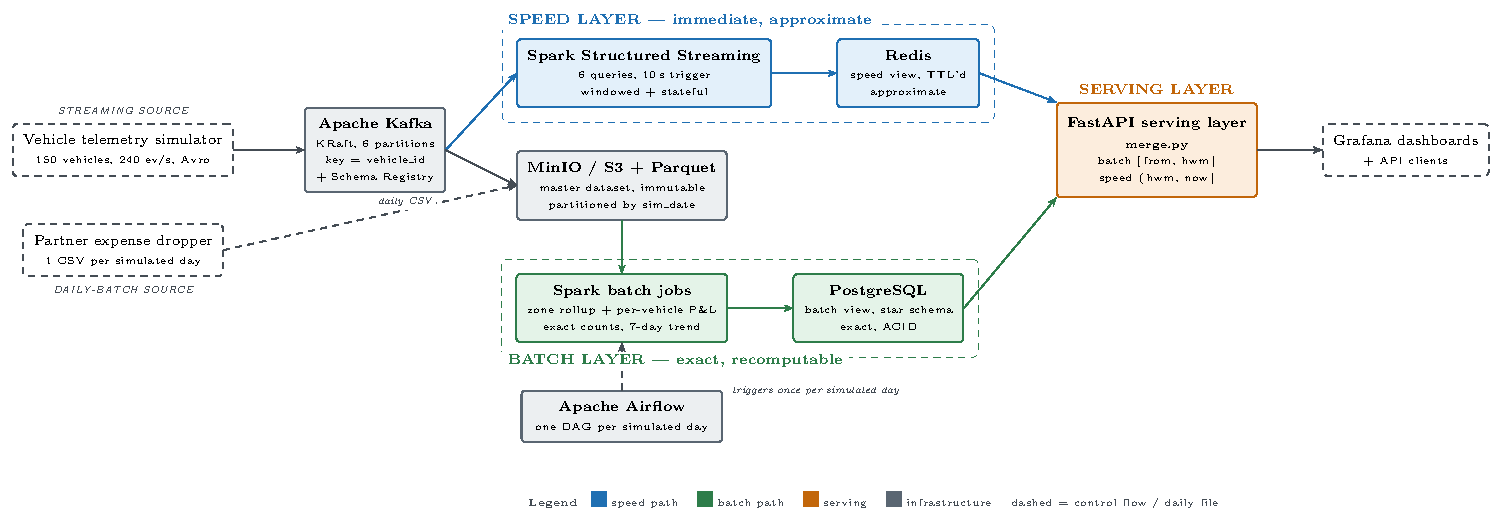
\includegraphics[width=\linewidth]{figures/D2-layered-architecture.pdf}
\caption{The layered architecture. Blue is the speed path, green the batch path,
grey shared infrastructure, orange the serving layer where the two are reconciled.
Note that the daily expense file bypasses Kafka entirely --- it is written straight
to object storage, because a once-a-day reference feed is not an event stream.}
\label{fig:d2}
\end{figure}

Four properties of Figure~\ref{fig:d2} carry the design:

\textbf{One log, three independent consumers.} Kafka is a persisted, append-only log
rather than a queue, so the same telemetry records feed the master-dataset writer, the
windowed aggregations and the stateful idle detector. Each has its own offsets and
fails alone: a Redis outage does not stop Parquet writes.

\textbf{The master dataset is immutable and append-only.} The batch layer recomputes
\emph{from} it and never edits it, which is what makes a restatement a recomputation
rather than a repair, and what makes any past day reproducible on demand.

\textbf{Zone is derived at read time, not stored.} Telemetry lands as raw validated
events; the zone is computed from latitude and longitude by the same shared function
in both layers. Baking a zone identifier into Parquet would freeze today's zone grid
into the historical record, and a redrawn grid could never be applied retrospectively.

\textbf{The two paths meet in exactly one place} --- \texttt{merge.py} in the serving
layer, described next.

\subsection{The merge boundary}
\label{sec:merge}

\begin{figure}[H]\centering
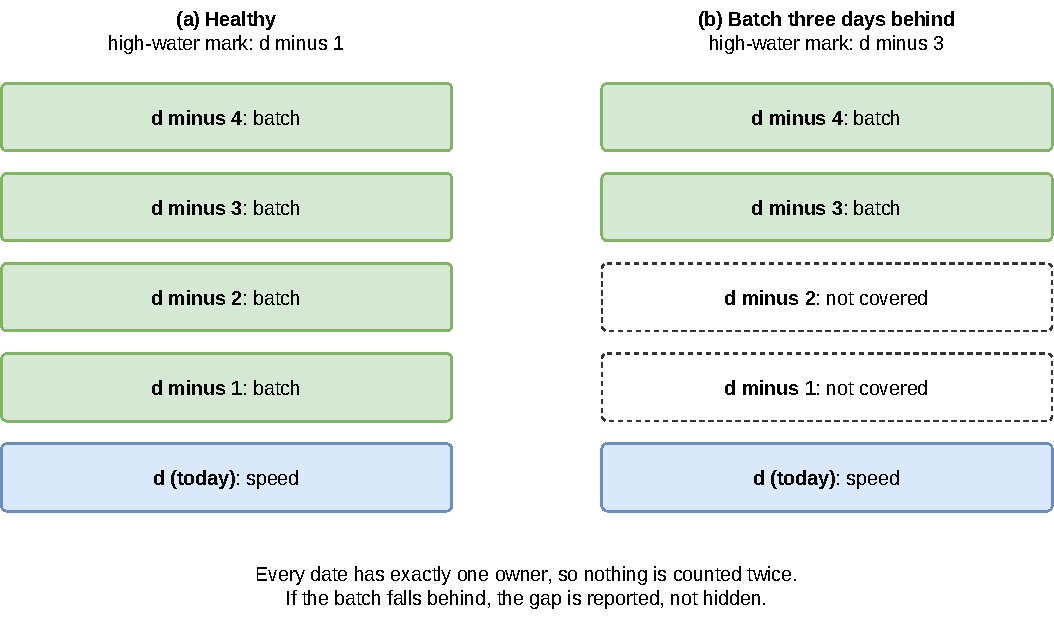
\includegraphics[width=0.74\linewidth]{figures/D4-merge-boundary.pdf}
\caption{The reconciliation rule. Half-open intervals mean the watermark date belongs
to exactly one side, so no date is double-counted and none is dropped.}
\label{fig:d4}
\end{figure}

The batch layer maintains a single-row table, \texttt{mart.batch\_high\_water\_mark},
recording the last simulated date it has fully processed. The serving layer reads it
and applies one rule:

\callout{The merge rule}{%
Batch serves $[\,\text{from},\ \text{hwm}\,]$ --- watermark \textbf{included}.\\
Speed serves $(\,\text{hwm},\ \text{now}\,]$ --- watermark \textbf{excluded}.\\[3pt]
The boundary date belongs to exactly one side, so there is provably no overlap and no
gap. Every row carries \texttt{source} and \texttt{exact}; the envelope carries a
plain-English \texttt{consistency} string.}

The watermark advances inside the same database transaction as the facts it
describes, so it can never claim a day whose data has not committed.

Two behaviours were added after the design met reality. First, because Redis holds
only the current window and not a per-date history, a batch layer that falls more than
one simulated day behind leaves dates that \emph{neither} view can answer for. Rather
than silently returning fewer rows --- which would make a lagging pipeline look like a
quiet week --- the response lists them in \texttt{uncovered\_dates} and names the gap
(Figure~\ref{fig:d4}b). Second, a requested date in the \emph{future} is reported
differently from one in that gap, because describing a not-yet-simulated date as
``the batch layer is behind'' would send somebody hunting a fault that does not exist.

\subsection{Event path}

\begin{figure}[H]\centering
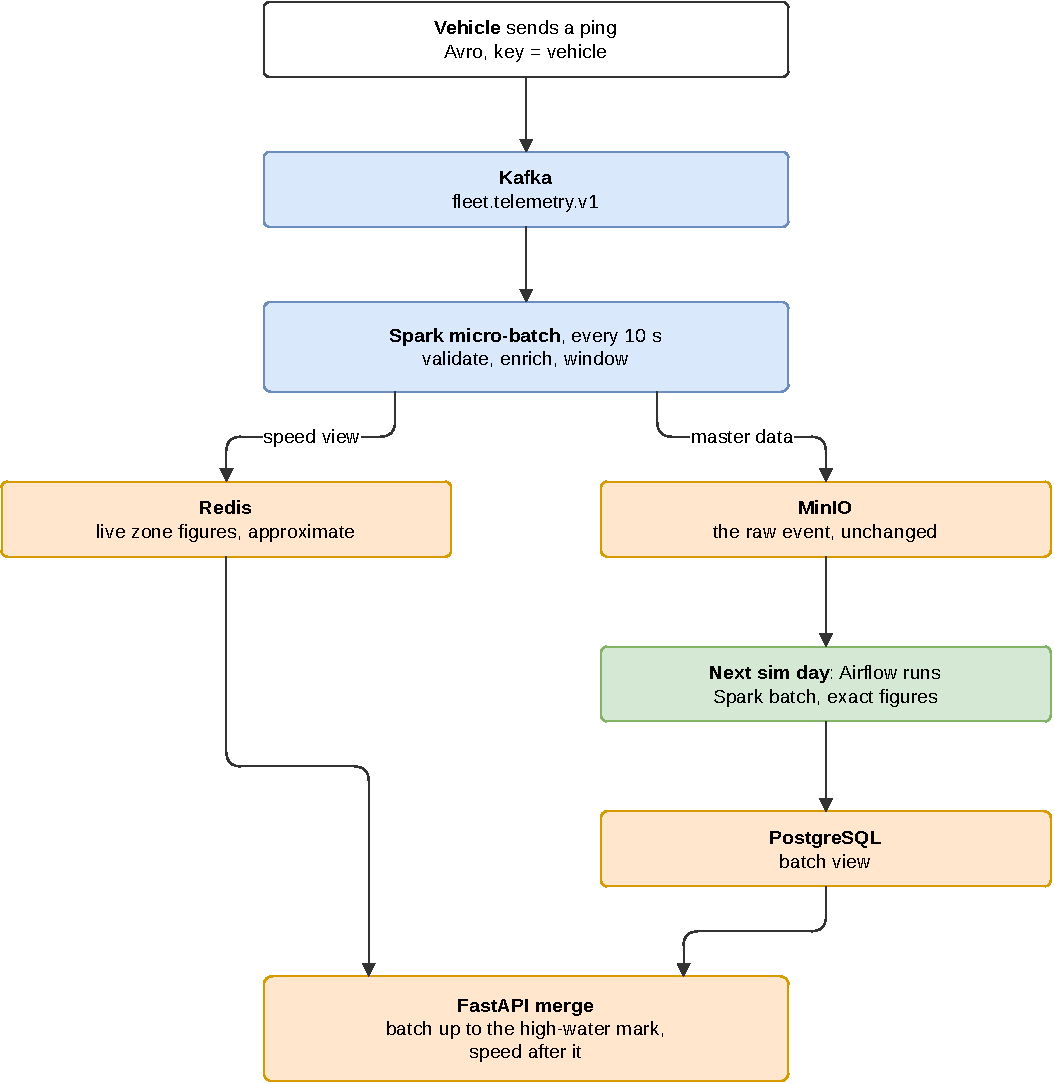
\includegraphics[width=0.84\linewidth]{figures/D3-event-sequence.pdf}
\caption{One telemetry event, end to end, with measured latencies. The fork is the
architecture: the same event is aggregated approximately within seconds and retained
verbatim for exact recomputation a simulated day later.}
\label{fig:d3}
\end{figure}

% ===========================================================================
\section{Technology Stack}

Each choice is justified against \emph{this} scenario rather than general popularity,
and the trade-off accepted is stated alongside it --- that column is what turns a list
into a justification.

\begin{table}[H]\centering\scriptsize
\begin{tabularx}{\linewidth}{@{}llXX@{}}
\toprule
\textbf{Layer} & \textbf{Chosen} & \textbf{Decisive reason for this scenario} & \textbf{Trade-off accepted} \\
\midrule
Ingestion & Kafka (KRaft) & Per-vehicle ordering via \texttt{vehicle\_id} partition key; one log, several independent consumers & \texttt{RF=1}: no fault tolerance at demo scale \\
Serialization & Avro + Schema Registry & Schema will evolve; 40--60\,\% smaller than JSON at 240\,ev/s & Harder to debug; an extra container \\
Speed processing & Spark Structured Streaming & \textbf{Same engine as the batch layer}, so one shared \texttt{transforms/} package answers the ``multiple codebases'' critique & Micro-batch latency floor \\
Speed store & Redis & Point lookups only; native TTL makes the transient view self-expiring & Not durable --- deliberately \\
Master dataset & MinIO + Parquet & Immutable partitions give deterministic, idempotent restatements; partition and column pruning & No ACID on the lake \\
Batch processing & Spark (batch) & Shares code with the speed layer; handles the wide join & JVM start-up per DAG run \\
Batch store & PostgreSQL star schema & ACID for financial figures; window functions for the rolling trend; transactional watermark & Holds aggregates only, by design \\
Orchestration & Airflow & File sensing, retries, branching, and a UI that makes health visible & Heaviest component \\
Serving & FastAPI & Somewhere for the merge logic to live and be tested & Custom code to defend \\
Dashboards & Grafana & Provisioned as code, reproducible from a clean clone & Less bespoke than a hand-built UI \\
Metrics & Prometheus + Pushgateway & PromQL expresses the required alert rules directly & Pushgateway is a known anti-pattern --- see \S\ref{sec:obs} \\
Alerting & Alertmanager & Real routing, grouping and inhibition & Another container \\
Logging & \texttt{structlog} $\rightarrow$ JSON & Structured logging with an enforced field schema & --- \\
\bottomrule
\end{tabularx}
\caption{Technology stack with per-component justification.}
\end{table}

Three choices are worth expanding, being the ones most open to challenge.

\textbf{Spark over Storm, Flink or Kafka Streams.} Not throughput --- any of them
handles 240\,events/s. Spark is the only one of the four that runs the \emph{same
code} in streaming and batch mode, and since this project's answer to the ``multiple
codebases'' criticism is a single shared transforms package, an engine that could not
execute that package in both modes would have cost the architectural argument.

\textbf{Redis for the speed view} was chosen partly \emph{because} it is not durable:
the view must be disposable for the fault-tolerance argument in \S3.5 to hold, and a
native TTL makes expiry a property of the store rather than a cleanup job that might
not run.

\textbf{Parquet on object storage rather than a database} for the master dataset,
because immutability is the requirement. A database invites updates; an append-only
partition layout makes ``recompute that day'' the only available correction, which is
the discipline the restatement argument depends on.

\callout{Honesty about scope}{%
Kafka, Spark, Airflow, PostgreSQL and the NoSQL family Redis belongs to were covered
in the module. MinIO/S3, Parquet, Prometheus, Grafana and Alertmanager were not; they
are deliberate extensions and are introduced as such rather than presented as taught
material.}

% ===========================================================================
\section{Implementation}

\subsection{Simulated sources}

Two Python sources, matching the brief's requirement for one streaming and one
daily-batch input. The telemetry simulator drives 150 vehicles through a state machine
(\texttt{idle} $\rightarrow$ \texttt{enroute} $\rightarrow$ \texttt{on\_trip}) across
a 12-zone grid with diurnal demand, emitting Avro every 3 simulated minutes at a
sustained 240\,events/s. The expense dropper writes one CSV per simulated day
straight to object storage --- never through Kafka --- and deliberately exercises the
awkward cases: a late file, a missing file, and \textbf{a restatement of a previous
day}, which is what makes the reprocessing argument demonstrable rather than
rhetorical.

The simulator also injects a known defect rate ($\approx$1\,\%) of malformed events:
negative fares, null coordinates, implausible speeds, out-of-bounds positions and
future timestamps. This is not decoration --- it is the control that makes the
dead-letter path measurable, as \S\ref{sec:results} shows.

\subsection{Ingestion}

\textbf{The partition key is the most important decision in this layer, and the
business logic dictates it.} Idle detection is stateful per vehicle: the detector must
observe \texttt{on\_trip} $\rightarrow$ \texttt{idle} $\rightarrow$ \texttt{idle} in
that order. Kafka guarantees ordering within a partition, not across partitions, so
keying by \texttt{vehicle\_id} places one vehicle's whole history on one partition and
the state machine sees a correctly ordered sequence. Any other key would break the
feature.

Avro with a Schema Registry provides the serialization contract, using the Confluent
wire format (a magic byte plus a four-byte schema id) so that producer and consumer
can evolve independently.

\subsection{Speed layer}

Six independent Structured Streaming queries share one source topic, each with its own
consumer group and checkpoint: master-dataset writer, dead-letter path, zone activity,
zone earnings, the stateful idle detector, and per-vehicle live state.

Two subtleties are worth recording. \emph{Activity and earnings must be separate
queries}, because Structured Streaming permits only one aggregation per query --- a
real cost of the correct answer, stated rather than hidden. And \emph{revenue must be
computed from a trip-deduplicated stream}: \texttt{fare} is the trip's fare repeated
on every ping, so summing it naively inflates revenue by the ping count. That defect
was found only by comparing total revenue against the distinct trip count; nothing
raised an error.

\subsection{Batch layer}

Two Spark jobs run per simulated day. The zone-hourly job computes exact per-zone,
per-hour facts using \texttt{countDistinct} where the speed layer uses
\texttt{approx\_count\_distinct} --- the two sit in the same source file, so the
accuracy trade-off is visible in twenty lines rather than argued over three
paragraphs. The profitability job reconstructs trips, computes distance by haversine
over consecutive GPS positions, \texttt{full\_outer}-joins the expense file
(handling matched, missing-expense and missing-telemetry cases), and derives the
7-day rolling average and trend slope.

Distance is recomputed from our own GPS trace rather than trusted from the partner's
odometer, so the system holds an independent measurement to reconcile against --- which
is the point of having two sources at all.

\subsection{Orchestration}

One DAG, \texttt{fleet\_daily\_reconciliation}, runs every 5 real minutes --- one
simulated day. It resolves the simulated date from the shared clock rather than
Airflow's \texttt{logical\_date} (the two are unrelated; using Airflow's would process
the wrong partition on every run), snapshots the speed view, senses and validates the
expense file, branches on the result, runs both Spark jobs, verifies the watermark
advanced, and computes the speed-versus-batch delta.

No transformation logic lives in the DAG file; an AST-based test enforces it. Logic in
a DAG only runs under a scheduler, so it escapes the unit suite and becomes a second,
untested copy of the pipeline --- reproducing inside our own orchestration exactly the
``multiple codebases'' problem Lambda is criticised for.

% ===========================================================================
\section{Observability Design}
\label{sec:obs}

The brief asks what is measured, how, and why. The \emph{why} column is the one that
matters, so it is filled in for every row.

\begin{table}[H]\centering\scriptsize
\begin{tabularx}{\linewidth}{@{}lXX@{}}
\toprule
\textbf{What} & \textbf{How} & \textbf{Why} \\
\midrule
Ingestion rate, errors, backpressure & \texttt{prometheus\_client} in the producers, scraped on \texttt{:8001}/\texttt{:8002} & If this is zero, nothing below it means anything --- every other panel looks calm because there is no traffic \\
Injected defect rate & Counter by defect type & The \emph{control} for the dead-letter path: what goes in must come out \\
Simulated clock drift & Gauge per container & Two services disagreeing about the date invalidates every windowed aggregate downstream \\
Streaming query progress & \texttt{StreamingQueryListener} $\rightarrow$ Pushgateway & See below --- it is the \emph{only} liveness signal these queries have \\
Micro-batch duration, state rows, watermark lag & Same listener & A duration approaching the trigger means the next batch starts late and lag compounds \\
Sink writes and errors & Counters in each \texttt{foreachBatch} & A sink failing silently is how the speed view goes stale while everything looks healthy \\
Batch watermark age & Gauge, set by the serving layer & A stopped batch layer has \emph{no other symptom} \\
Merge boundary crossings & Counter & A flat zero means the reconciliation was never exercised \\
Degraded responses & Counter by missing store & Degrading is correct behaviour --- but a sustained rate means we are running on half the architecture \\
API latency and request rate & \texttt{prometheus-fastapi-instrumentator} & p95 rising while p50 is flat indicates one slow store, not a slow API \\
Structured logs & \texttt{structlog} JSON, every stage & A guard processor rejects reserved field names, which previously overwrote log levels silently \\
\bottomrule
\end{tabularx}
\caption{What is measured, how, and why.}
\end{table}

\subsection{Consumer lag cannot measure Structured Streaming}

This is the section's most important point, and it was learned the hard way.

The obvious way to monitor a Kafka consumer is consumer-group lag. \textbf{It does not
work for Structured Streaming.} These queries checkpoint their own offsets and never
commit to a consumer group, so lag reads zero whether a query is keeping up or has
been dead for hours. On the running system, \texttt{kafka-consumer-groups --list}
returns \textbf{no groups at all} --- which is why the consumer-lag panel in
Figure~\ref{fig:health} is empty, and why that empty panel is left in place and
labelled rather than removed. The empty panel is the evidence.

An earlier attempt to force the metric to work by setting \texttt{kafka.group.id}
\emph{killed the dead-letter query} after roughly 4{,}500 micro-batches.

The signal that does work is the \textbf{age of the last progress timestamp} pushed by
a \texttt{StreamingQueryListener}. A query processing zero rows may be perfectly
healthy and idle; a query that has stopped emits no progress at all, and only the age
of that timestamp distinguishes the two. Pushgateway is a known anti-pattern for
long-lived jobs precisely because a pushed metric outlives the process that pushed it
--- mitigated here by alerting on the timestamp's age rather than on its value.

\subsection{Alerting, and an alert that could not fire}

Six rules, routed through Alertmanager, chosen so that each can be \emph{demonstrated}
firing rather than merely written. Business alerts about vehicles are kept separate
and flow through Kafka as data --- conflating ``a vehicle has been idle too long''
with ``the pipeline is down'' is how an on-call rota learns to ignore its own alerts.

The rule the brief asks for by name --- no data received in N minutes --- was written
first as:

\begin{center}\ttfamily\small
sum(rate(events\_produced\_total[2m])) == 0
\end{center}

It loaded cleanly and appeared in the Prometheus UI. The producer was then stopped,
and the alert \textbf{stayed inactive for six and a half minutes}.

The cause is worth stating plainly because it generalises: \textbf{absent is not
zero}. When the producer dies its scrape target goes down, the series goes stale and
disappears, and \texttt{sum(rate(...))} over no series returns an \emph{empty vector}.
Comparing an empty vector to zero yields an empty vector. The alert for ``no data
received'' was defeated by there being no data.

The fix was \texttt{or vector(0)}, which substitutes a literal zero when the series is
absent, plus a companion rule on \texttt{up == 0} --- a series Prometheus synthesises
for every configured target, and which therefore goes to zero instead of vanishing.
Post-fix the alert fires in \textbf{71 seconds} and resolves in \textbf{51}.

\subsection{Inhibition}

Stopping the producer raises eight alerts: one cause and seven consequences (five
stalled queries, one target down, one no-data). Alertmanager inhibition suppresses the
consequences so that on-call sees the cause. The first inhibition rule written
suppressed \emph{nothing}, because it matched \texttt{severity="warning"} while the
consequential alerts are \texttt{critical}. Corrected to a causal chain, the same
incident now presents as \textbf{five alerts reduced to one actionable}.

% ===========================================================================
\section{Results}
\label{sec:results}

\subsection{The business question, answered}

\begin{figure}[H]\centering
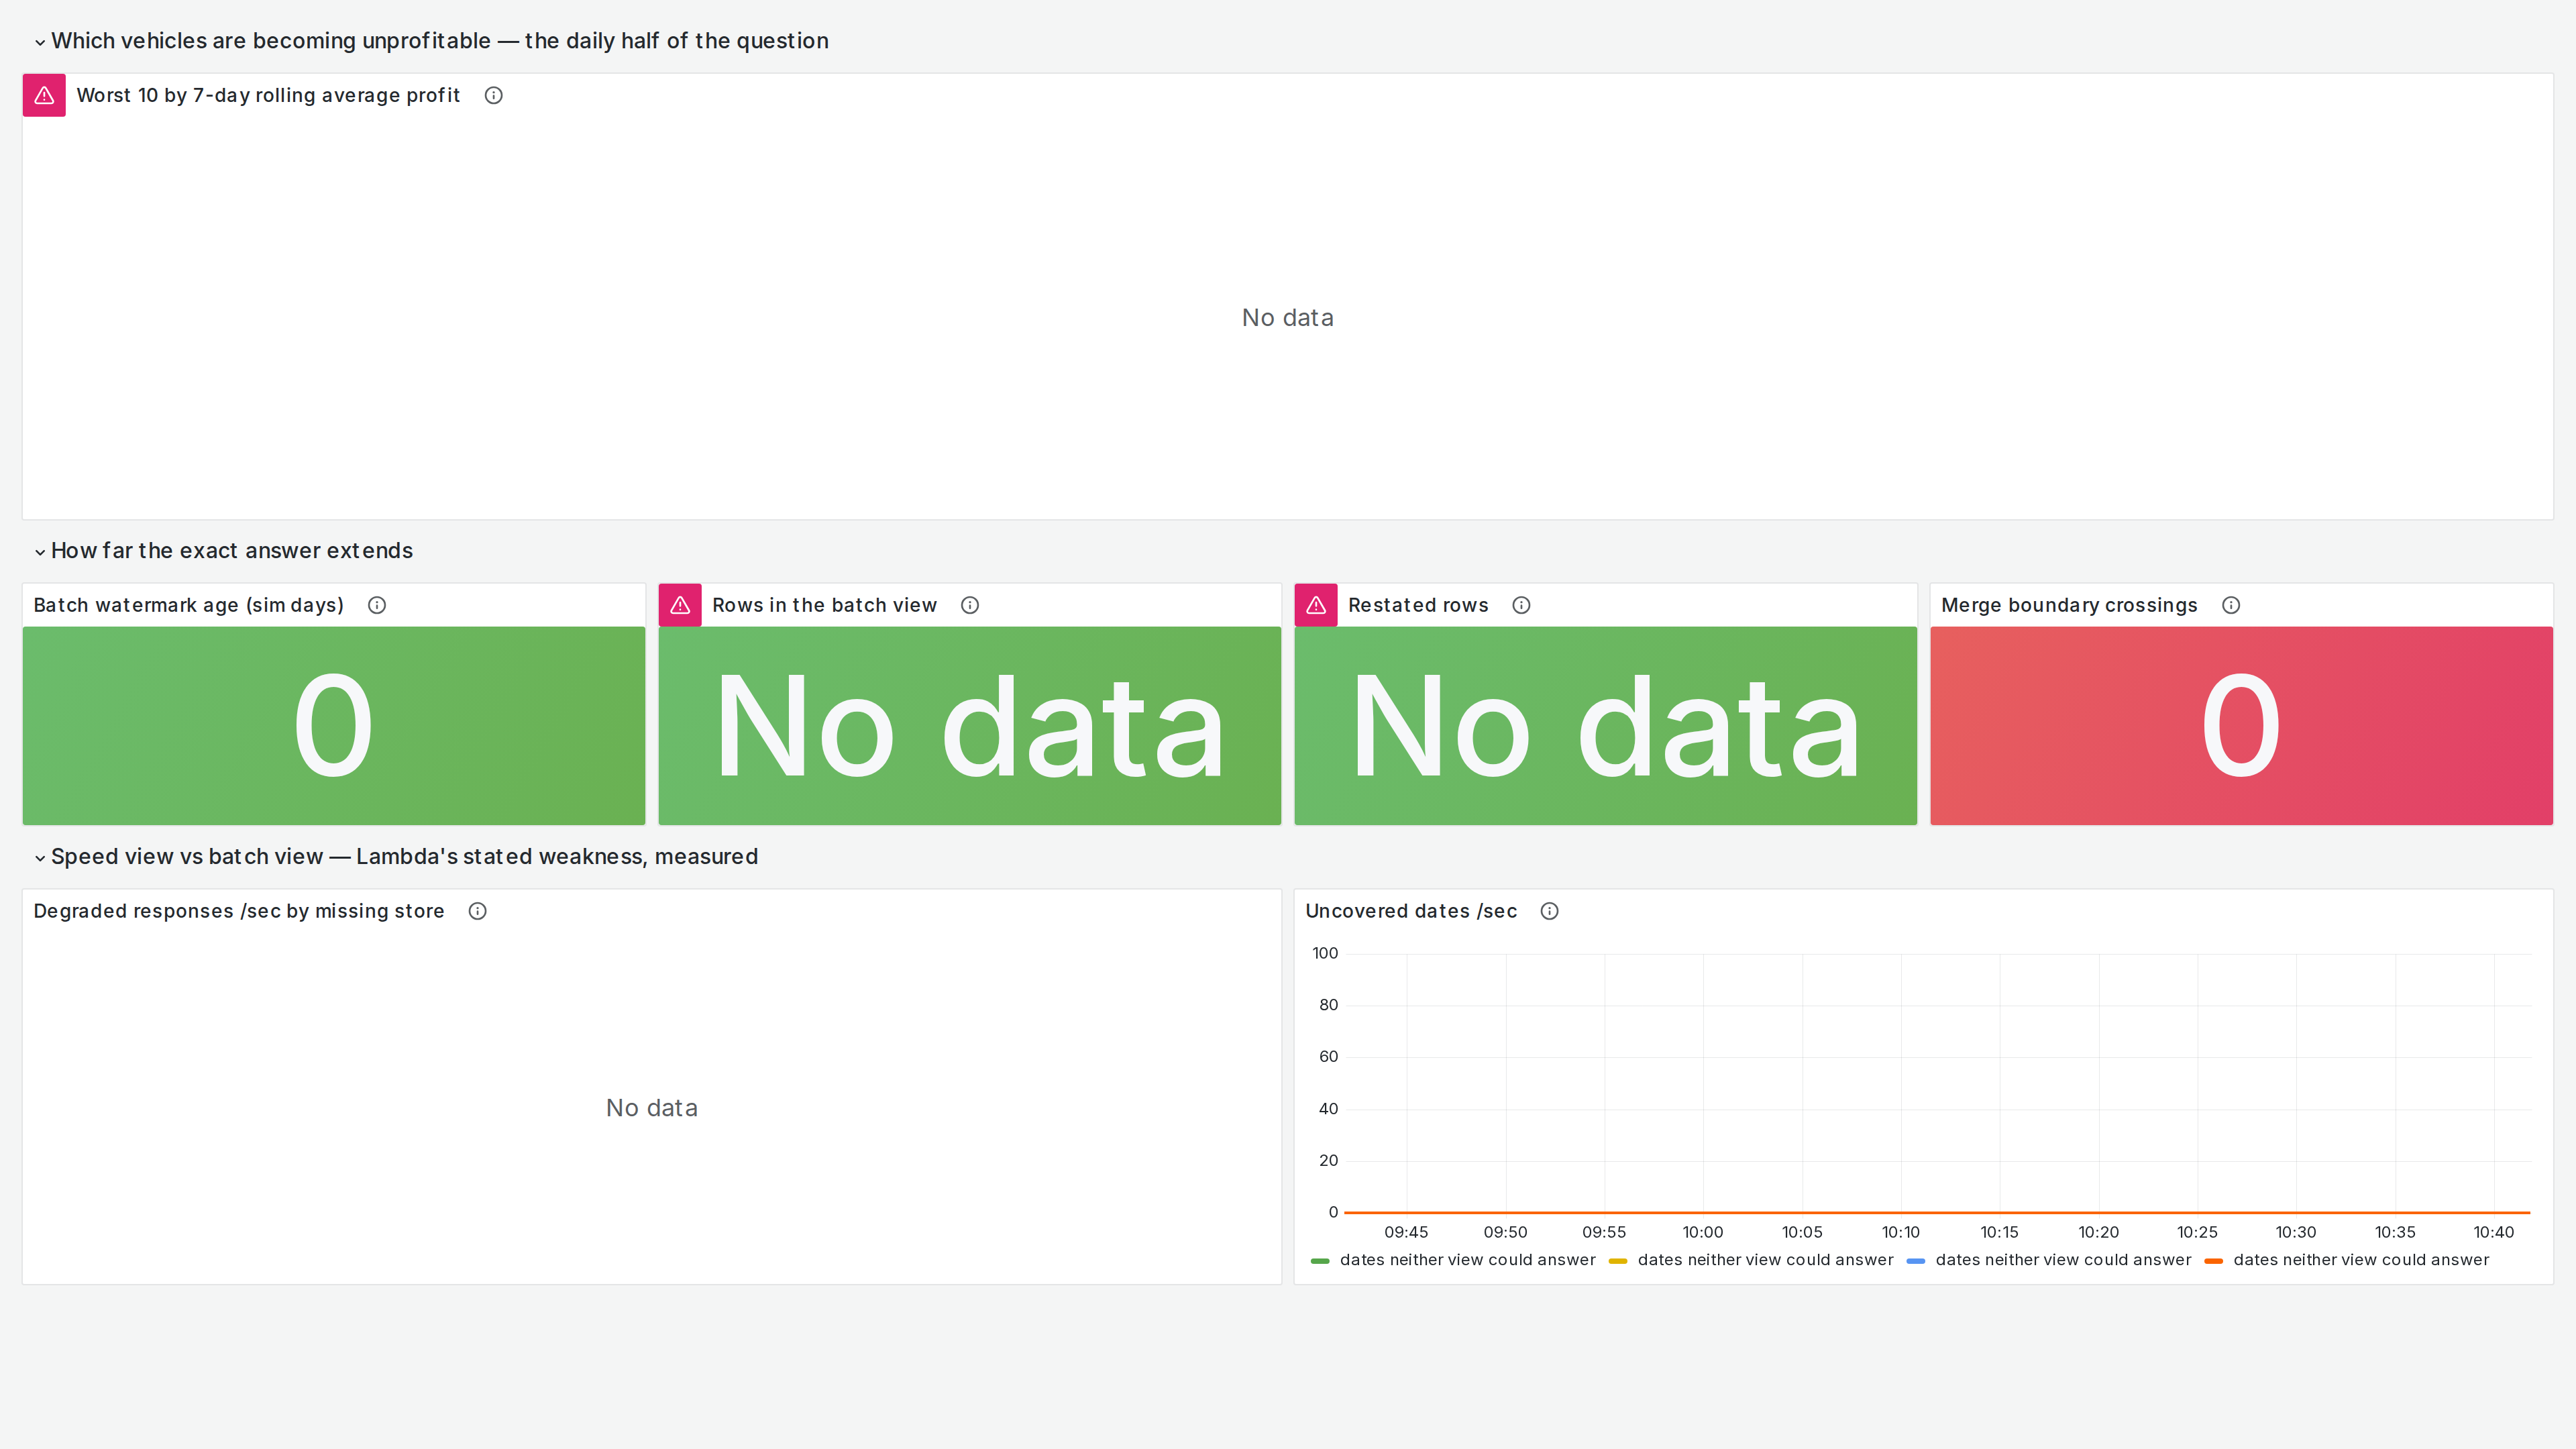
\includegraphics[width=0.64\linewidth]{figures/R2-batch-reconciliation.png}
\caption{Question B answered: vehicles ranked by 7-day rolling average profit, with
classification, trend slope and margin. Ordering is by the rolling average rather than
today's profit, because one bad day is noise --- a vehicle with a single long deadhead
must not outrank one that has lost money all week.}
\label{fig:batch}
\end{figure}

\begin{figure}[H]\centering
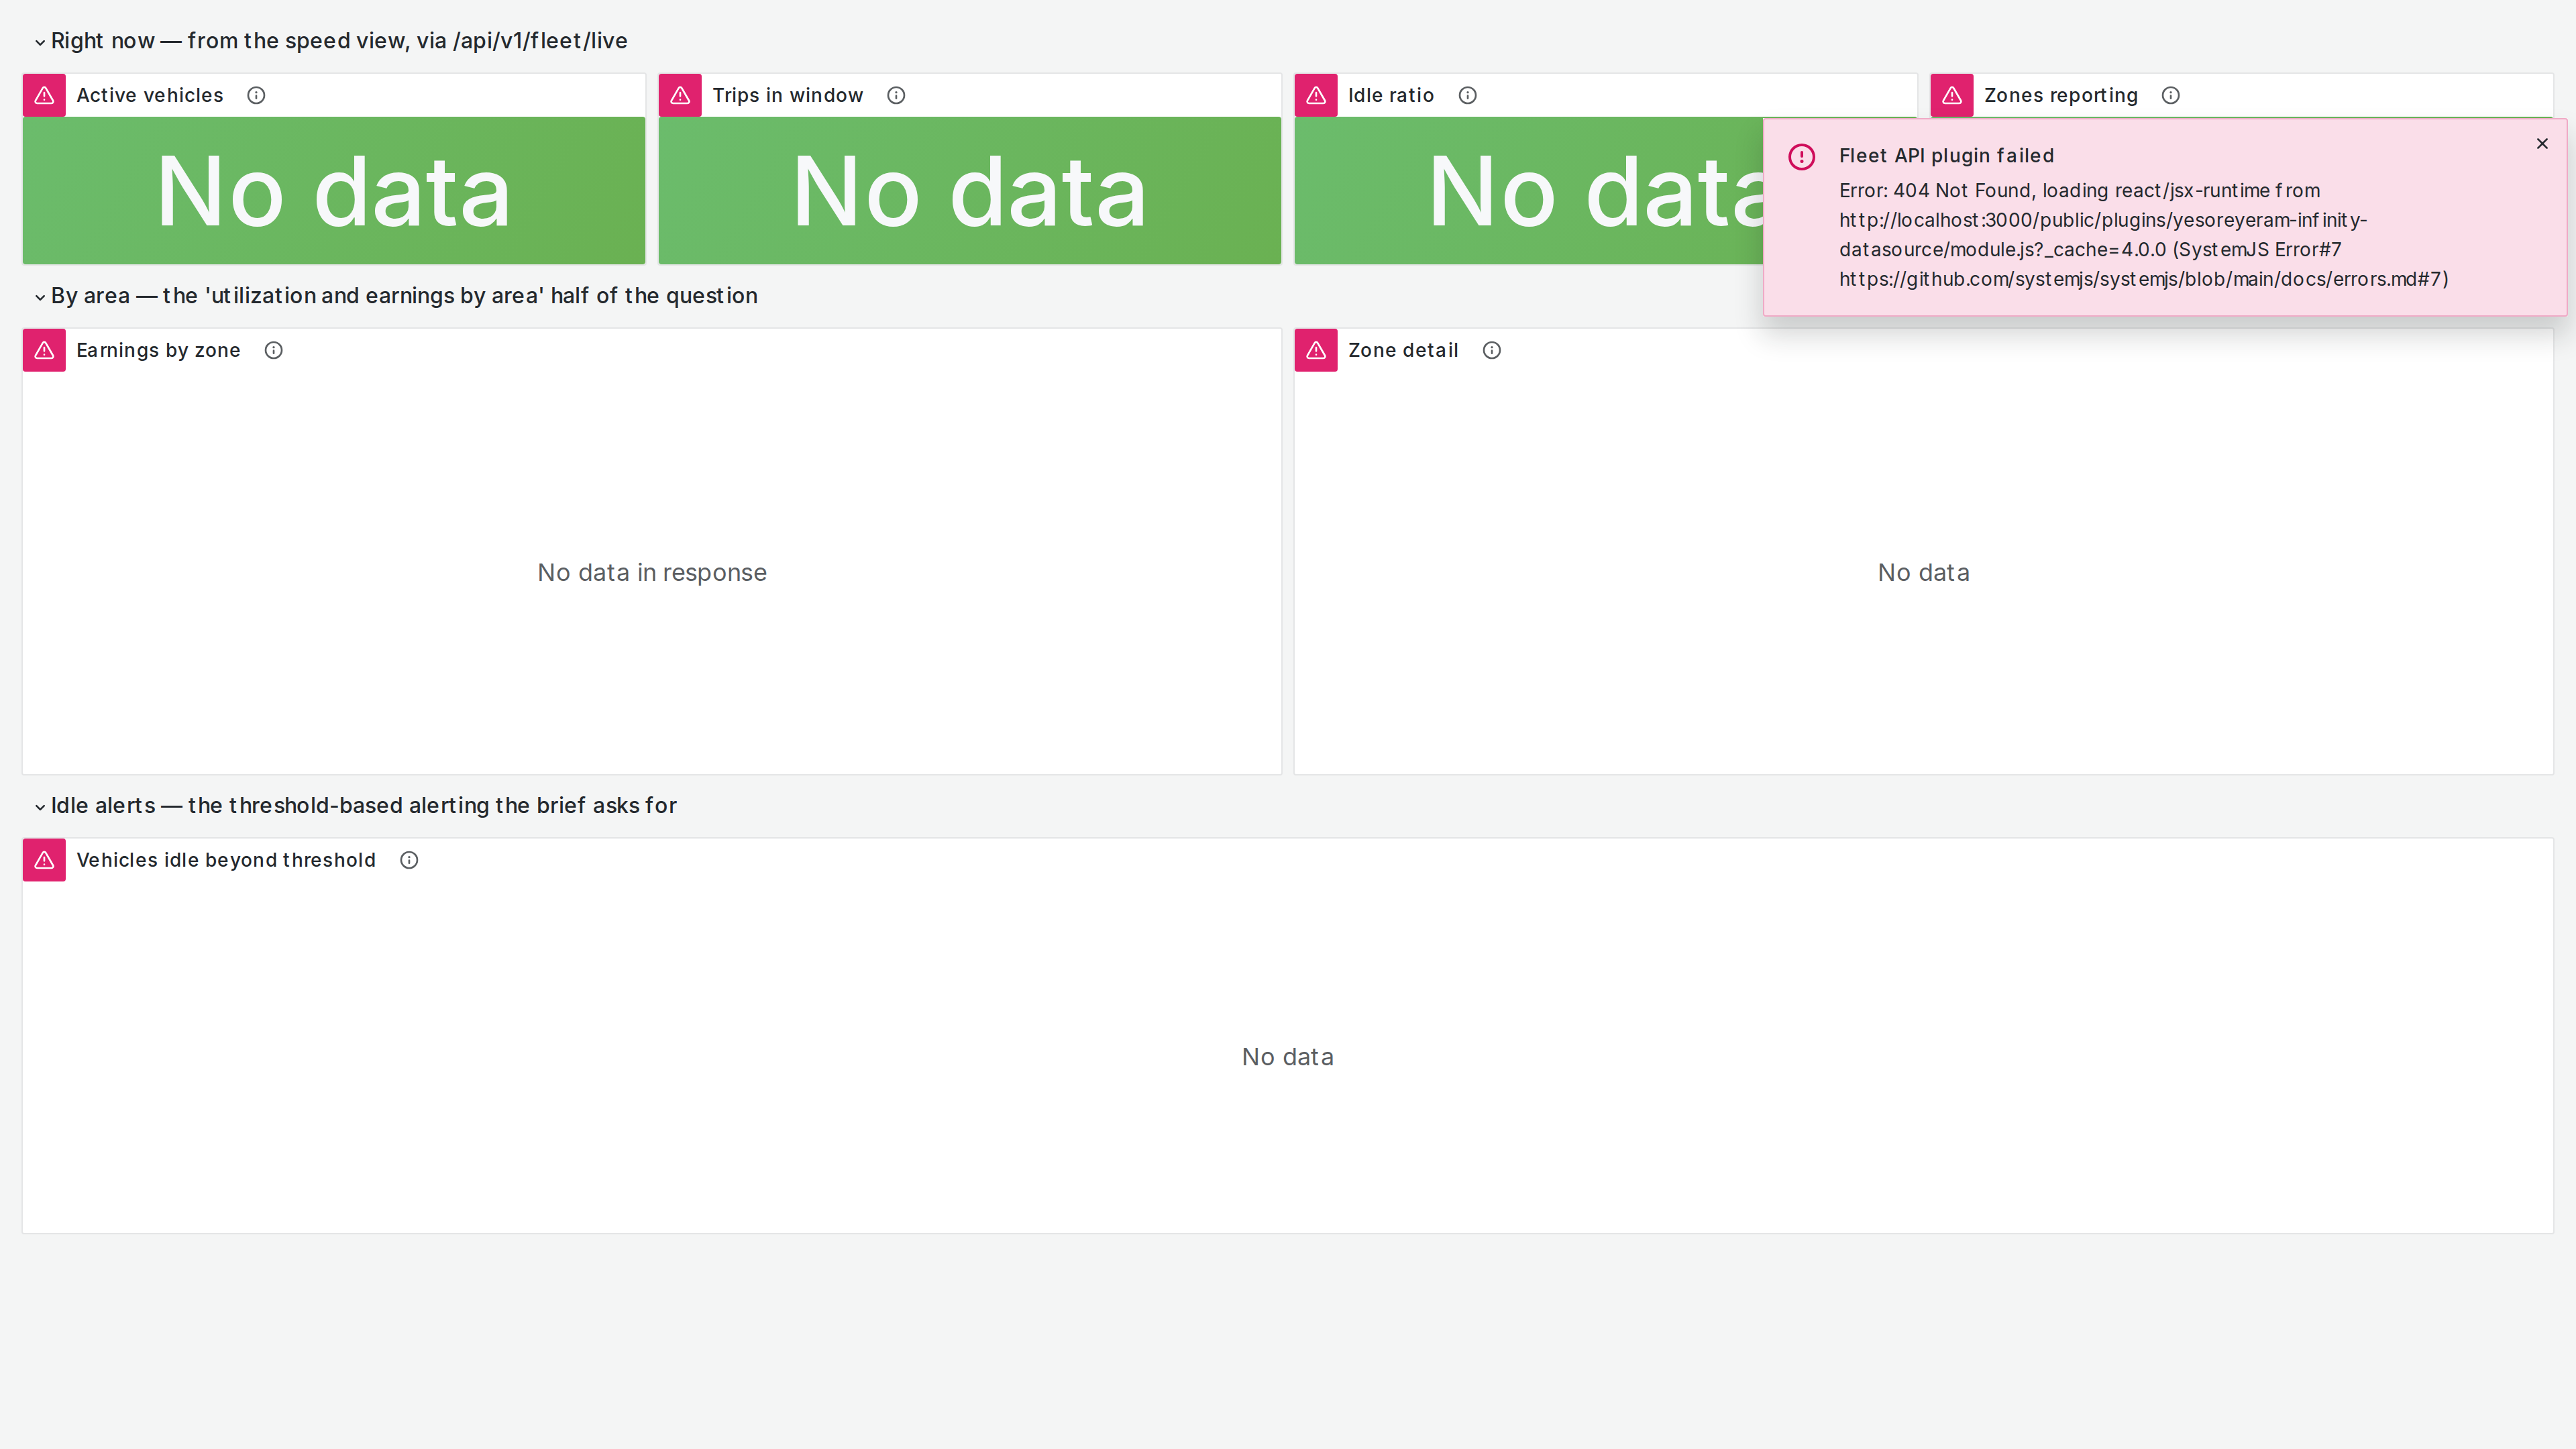
\includegraphics[width=0.64\linewidth]{figures/R1-fleet-operations.png}
\caption{Question A answered: live utilization, idle ratio and earnings by zone. Every
panel is served through the project's own API rather than by reading Redis directly,
so a panel that breaks is telling the truth about the serving layer.}
\label{fig:ops}
\end{figure}

\subsection{Correctness evidence}

The strongest evidence is not that the system runs, but that two independent
computations agree. Per-vehicle revenue is summed from a trip-deduplicated join
grouped by vehicle; per-zone earnings are summed from a different deduplication rule
grouped by zone and hour. Different code paths, different groupings:

\begin{table}[H]\centering\small
\begin{tabular}{@{}lrrr@{}}
\toprule
\textbf{Simulated date} & \textbf{P\&L revenue} & \textbf{Zone earnings} & \textbf{Delta} \\
\midrule
2026-03-01 & 46{,}878.04 & 46{,}878.04 & \textbf{0.00} \\
2026-03-02 & 50{,}920.07 & 50{,}920.07 & \textbf{0.00} \\
2026-03-03 & 49{,}736.90 & 49{,}736.90 & \textbf{0.00} \\
2026-03-04 & 49{,}808.52 & 49{,}808.52 & \textbf{0.00} \\
\bottomrule
\end{tabular}
\caption{Two independent paths to one number, agreeing to the penny.}
\end{table}

A second control: the simulator injects a $\approx$1\,\% defect rate, and the
dead-letter topic holds \textbf{41{,}915 of 3{,}830{,}077} messages ---
\textbf{1.09\,\%}. The expected answer was known before the measurement, which is what
makes it evidence rather than a statistic. Similarly, the vehicle registry topic holds
exactly \textbf{150} records for 150 vehicles.

\subsection{The merge, and graceful degradation}

Requesting a range spanning the watermark returned 48 rows --- 36 batch, 12 speed ---
with \textbf{every date owned by exactly one side}: no date appeared twice, none was
missing. Degradation was tested by stopping stores:

\begin{table}[H]\centering\small
\begin{tabularx}{\linewidth}{@{}llX@{}}
\toprule
\textbf{Scenario} & \textbf{HTTP} & \textbf{Response} \\
\midrule
Both stores up & 200 & 48 rows, \texttt{degraded: false} \\
Redis stopped & \textbf{200} & 36 batch rows, \texttt{X-Data-Degraded: true} \\
PostgreSQL stopped & \textbf{200} & speed rows; watermark reported \emph{unknown}, not ``cold start'' \\
Both stopped & \textbf{503} & names both stores; never a 500 \\
Restarted & 200 & \texttt{degraded: false}; pool reconnected unaided \\
\bottomrule
\end{tabularx}
\caption{One store down is a warning, not an outage. Only total loss fails.}
\end{table}

\subsection{Measured performance}

\begin{table}[H]\centering\small
\begin{tabular}{@{}lll@{}}
\toprule
\textbf{Measurement} & \textbf{Value} & \textbf{Against} \\
\midrule
Sustained ingestion & 240.2\,events/s & configured target 240 \\
Live-view freshness (p50 / p95) & \textbf{7.9\,s} / \textbf{23.6\,s} real & NFR-1 $<$30\,s --- \textbf{met} \\
API latency (p50 / p95 / p99) & 50 / 95 / 99\,ms & --- \\
PostgreSQL query latency, pooled & 8--15\,ms & 30--65\,ms unpooled \\
Batch job, one simulated day & 73\,s cold / 50\,s warm & --- \\
Airflow DAG run (mean / max) & 1\,min 51\,s / 4\,min 32\,s & 5-minute schedule \\
Alert detection / resolution & 71\,s / 51\,s & NFR-4 $<$3\,min --- \textbf{met} \\
Idempotent re-run & \textbf{0} restatements & NFR-3 --- \textbf{met} \\
\bottomrule
\end{tabular}
\caption{Measured on the running stack; none of these figures is estimated.}
\end{table}

\textbf{An honest capacity finding.} Micro-batch durations at p95 are 17.6\,s
(\texttt{q\_activity}), 17.7\,s (\texttt{q\_earnings}) and 21.7\,s (\texttt{q\_idle})
against a \textbf{10-second trigger}. Three of six queries therefore exceed their own
trigger interval at the tail, which is the direct cause of the 23.6\,s p95 freshness
above. The three affected are exactly the windowed and stateful ones; the stateless
pass-throughs stay well inside the trigger while processing more rows per second. The
honest answer to ``does it keep up?'' is: on average yes, at the tail no.

\subsection{Idempotency and restatement}

Re-running the batch layer for one simulated date, with the watermark standing at a
later date throughout:

\begin{table}[H]\centering\small
\begin{tabular}{@{}llr@{}}
\toprule
\textbf{Run} & \textbf{Job run id} & \textbf{$\sum$ restatement\_count} \\
\midrule
before & --- & 300 \\
A & new id & 450 \quad (+150, every row audited as republished) \\
B & \emph{same} id & \textbf{450} \quad (delta \textbf{0} --- idempotent) \\
\bottomrule
\end{tabular}
\caption{A re-run under the same job id changes nothing; a new id records the
restatement. The watermark never moved backwards.}
\end{table}

\begin{figure}[H]\centering
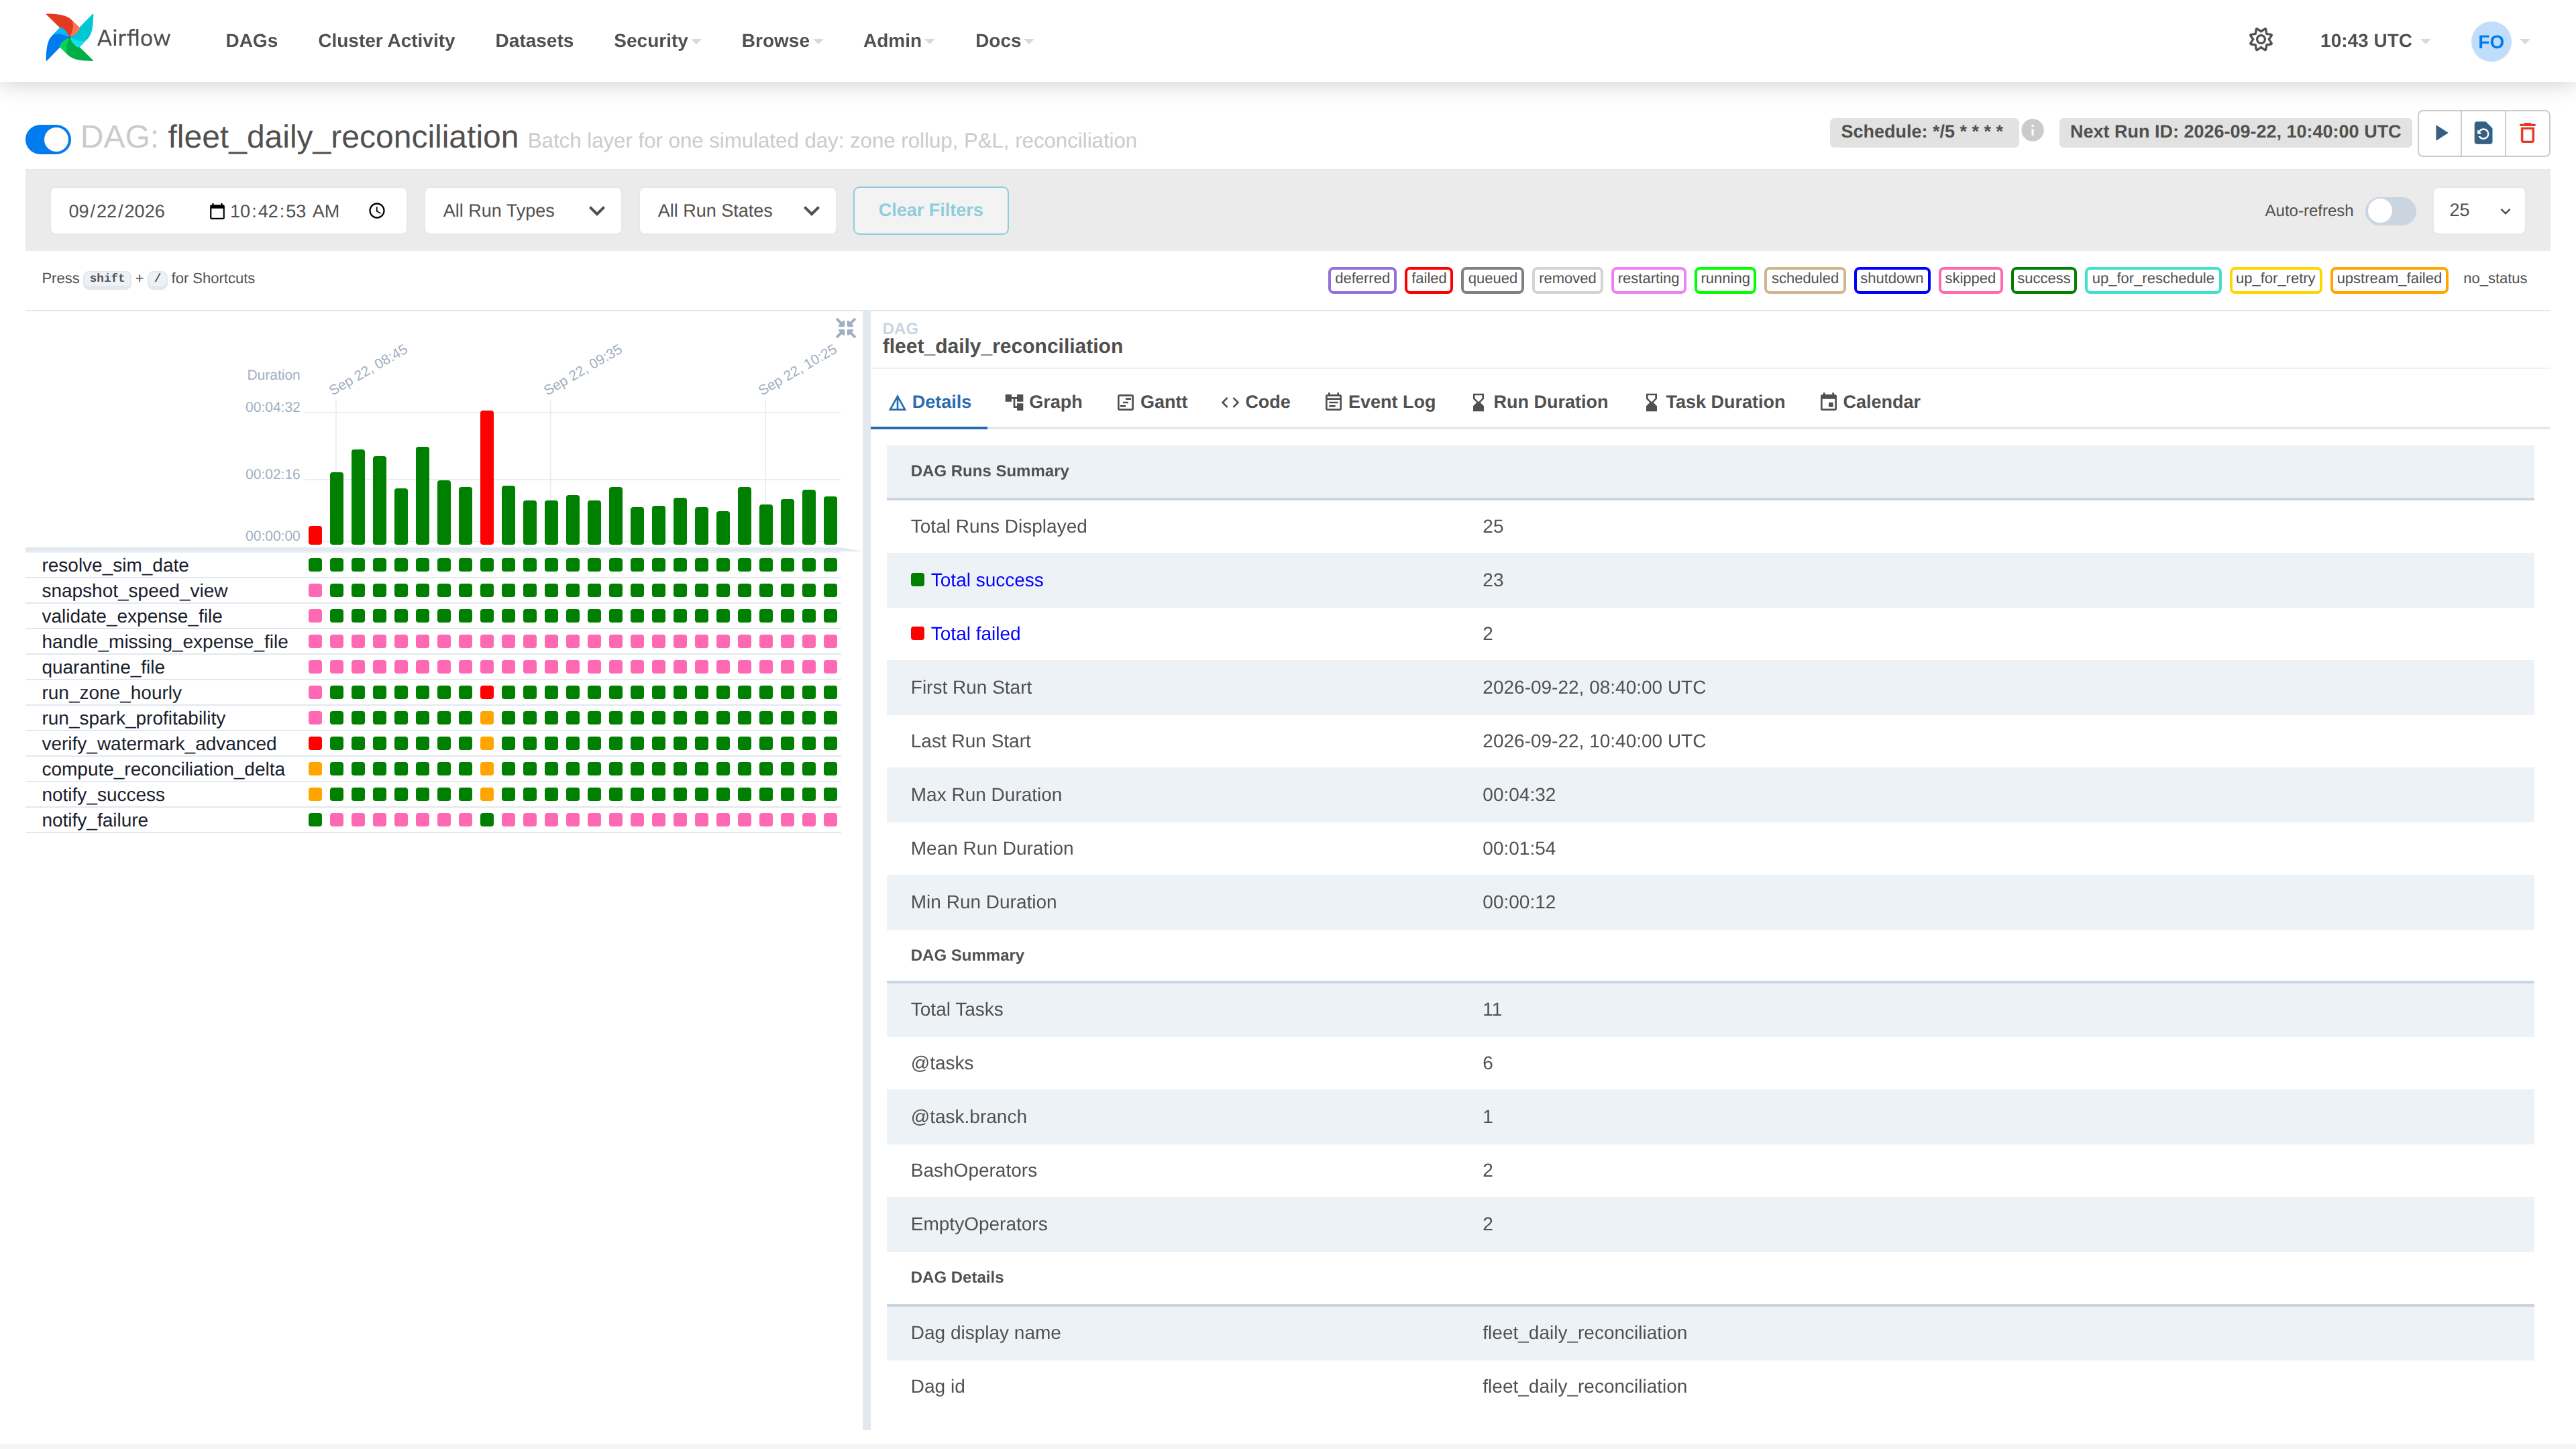
\includegraphics[width=0.64\linewidth]{figures/R4-airflow-grid.png}
\caption{The batch layer on schedule: 25 runs, 22 successful, mean 1\,min 51\,s. The
three failures are pre-fix runs discussed in \S\ref{sec:limits}.}
\label{fig:airflow}
\end{figure}

\begin{figure}[H]\centering
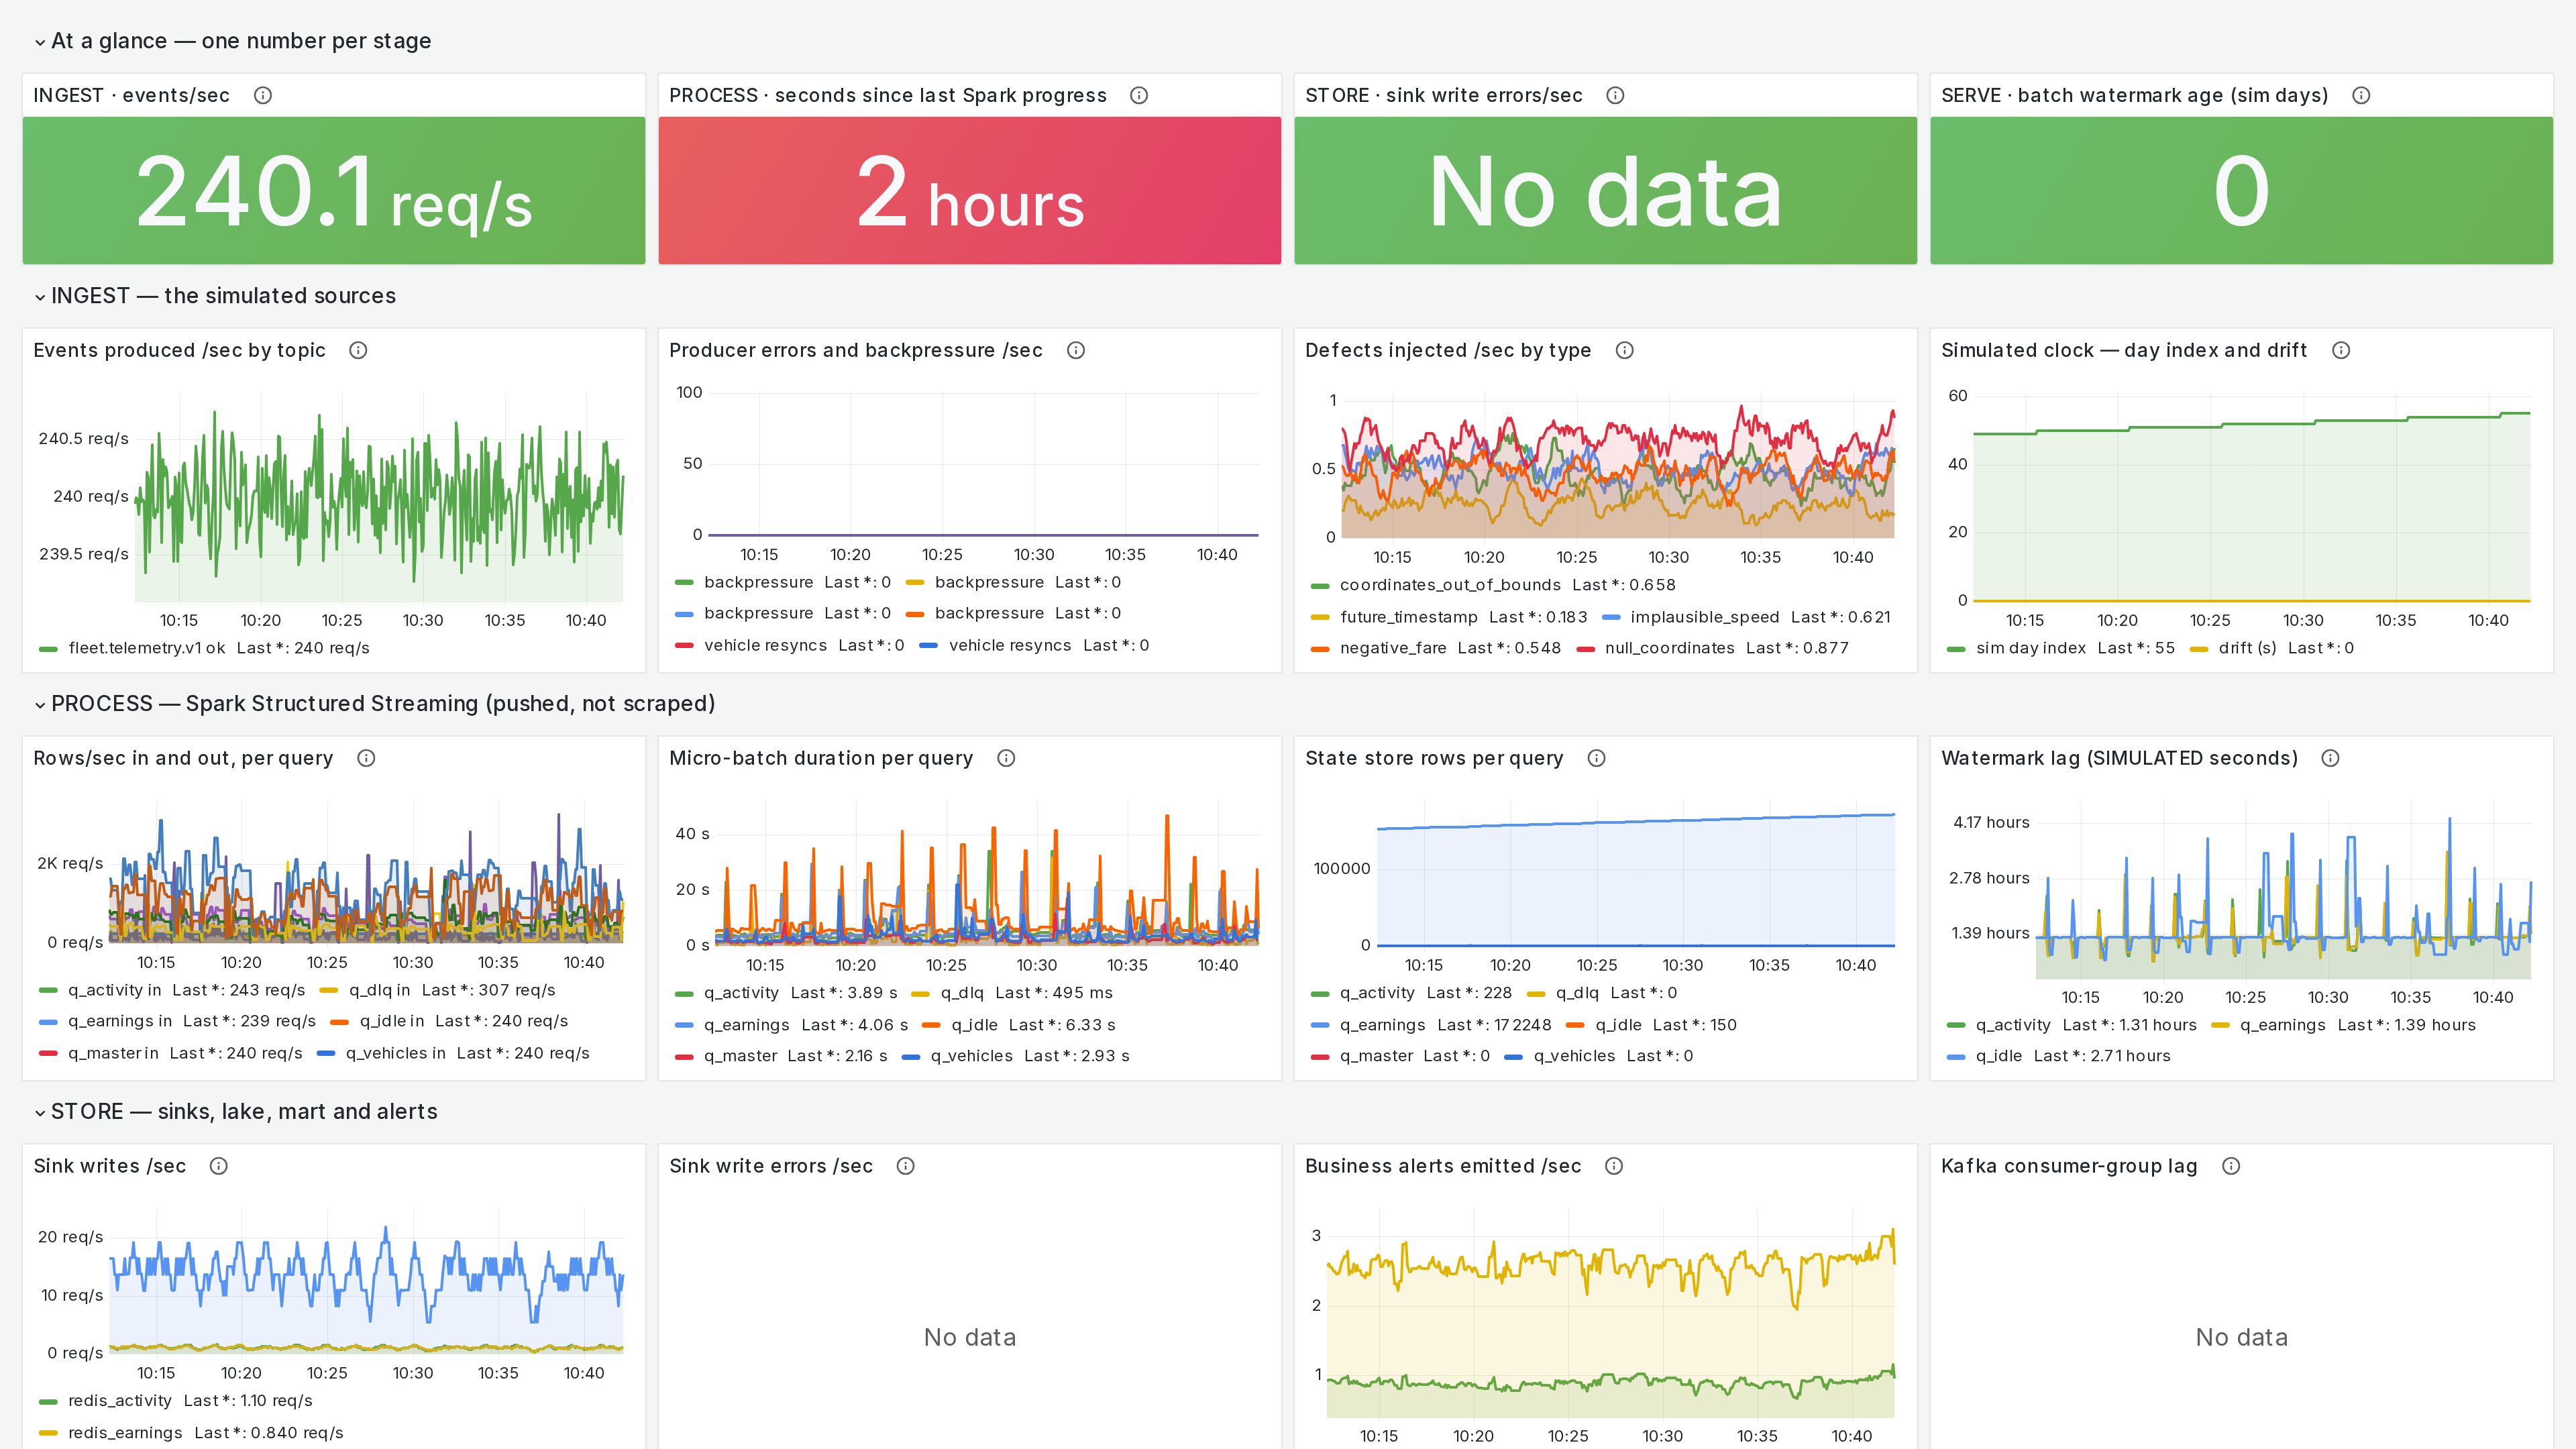
\includegraphics[width=0.64\linewidth]{figures/R10-pipeline-health.png}
\caption{Pipeline health across all four stages. The consumer-lag panel is empty by
design --- see \S\ref{sec:obs}.}
\label{fig:health}
\end{figure}

% ===========================================================================
\section{Limitations, Trade-offs and Production Scale}
\label{sec:limits}

\subsection{Every defect found was silent}

The most useful thing learned on this project is a pattern rather than a fact.
\textbf{Not one application defect announced itself.} None raised an exception, none
appeared in a log, and every one of them would have survived to a live demonstration
had the only check been ``is the pipeline running?''. A representative sample:

\begin{itemize}
\item Revenue was inflated 8.5$\times$ because \texttt{fare} repeats on every ping of
a trip. Found by comparing total revenue against the distinct trip count.
\item The speed layer started \textbf{two of six} streaming queries --- a default left
over from an earlier iteration --- so a fresh start produced no speed view at all.
Redis was simply empty, which looks exactly like a store that has not warmed up yet.
\item An Airflow branch skipped the \emph{entire} batch path, because a task with two
upstreams used the default trigger rule. The DAG went amber rather than red and the
only durable symptom was a watermark that never advanced.
\item The idle-alert feed deleted itself every 25 real seconds: a Redis TTL applies to
the whole key, so all 200 alerts vanished at once and reappeared on the next write.
Alerts were streaming into Kafka the entire time.
\item The Airflow web interface was \textbf{dead for three hours} after its workers
were out-of-memory killed. Nothing noticed, because the scheduler is a separate
container and kept running DAGs perfectly.
\end{itemize}

What caught all of them was the same technique: \textbf{comparing an output against an
independently known expected value}. Injected defects against dead-lettered count.
Revenue against distinct trips. Registry records against fleet size. Per-vehicle
revenue against per-zone earnings. A pipeline that merely runs tells you nothing; a
pipeline whose output can be checked against a number you already knew tells you
everything.

The corollary shaped the tooling: \textbf{a check that cannot fail is not a check}.
The screenshot script initially reported ten successes while two of its images were a
login page and a blank page, because its only test was whether the screenshot call
threw. The alert rule loaded cleanly and could never fire. A DAG integrity test passed
against zero DAGs. Each was fixed by making the check assert something it could get
wrong.

\subsection{Demo-scale simplifications}

Single Kafka broker with \texttt{replication.factor=1}, so a broker loss loses
unconsumed data. Retention reduced from the design value to roughly an hour. Spark in
\texttt{local[4]} rather than on a cluster --- the Structured Streaming semantics
(windowing, watermarking, checkpointing, state) are identical; what is not
demonstrated is task distribution across separate executor nodes. 150 vehicles rather
than several thousand. No authentication, TLS or ACLs anywhere, and default
credentials in the environment file. \textbf{At 240\,events/s this was never a
distributed-scale demonstration in any configuration}; it demonstrates architectural
correctness and pipeline behaviour, and the performance table in \S\ref{sec:results}
gives the scaling analysis in place of a scale test.

\subsection{Correctness and semantics}

End-to-end exactly-once is \textbf{not} achieved: the system is at-least-once with
idempotent sinks, which is why every sink overwrites rather than increments. Speed
layer distinct counts are HyperLogLog. Earnings in the live view lag by up to one trip
duration, because revenue is recognised at trip completion. Events later than the
30-simulated-minute watermark are dropped from windowed aggregates, though they still
reach the master dataset. There is no ACID on the lake --- a crashed writer can leave
a partial Parquet file, mitigated by the streaming commit log rather than eliminated.

\subsection{The reconciliation does not match its own prediction}

The design predicted a speed-versus-batch divergence of 1--3\,\% on counts and up to
8\,\% on earnings. Measured fleet-wide, it is not: \texttt{idle\_ratio}
\textbf{$-$9.3\,\%}, \texttt{earnings\_per\_min} $-$37.9\,\%, \texttt{trips\_per\_min}
$-$86.1\,\%.

Two genuine defects were fixed on the way to those numbers. The first comparison had a
\emph{unit mismatch} --- a 15-simulated-minute sliding window compared against a whole
batch day --- which produced a meaningless $\approx$99\,\% ``divergence''. The second
was keyed on \emph{when the orchestrator ran} rather than on the window the data
describes; the speed view lags the clock by about 93 simulated minutes (only
$\approx$19 real seconds at 288$\times$, but more than an hour in simulated time), so
one hour's speed reading was being compared against a different hour's batch figure.
Fixing that moved \texttt{idle\_ratio} from $+$23\,\% to $-$9.3\,\%.

The residual gap on the flow metrics is not a fault but a property: a once-daily
snapshot catches a \textbf{partially accumulated} sliding window, so point-in-time
sampling systematically under-reads. Per zone the snapshot recorded 0--3 trips where
the batch hour recorded 25--65. \texttt{idle\_ratio} is the only metric here that is
independent of window width --- it is a ratio, not a count --- and is therefore the
figure worth quoting.

Making this meaningful for flow metrics would require accumulating the speed view
across the day rather than sampling it once. That is future work, and it is named as
such rather than quietly omitted. \textbf{The measured result with an explanation is a
better answer than a prediction that was never tested would have been.}

\subsection{What is not implemented}

Stated plainly rather than left for a reader to discover. \textbf{Distributed tracing
was not implemented} --- the design called for OpenTelemetry and Jaeger with one span
per micro-batch, and this was cut for time. The observability story therefore rests on
structured logging, metrics and alerting, and a request cannot currently be followed
across process boundaries by a trace id. \textbf{The generated PDF daily report was
not implemented}; the brief asks for ``a consolidated report \emph{or} dashboard'' and
the provisioned Grafana dashboards discharge that requirement, but the rendered
document described in the design does not exist. Log aggregation (Loki) was likewise
not built.

One further operational limitation: \texttt{catchup=False} means simulated days missed
during an outage are never picked up automatically. This was observed --- the
watermark sat three simulated days behind after a deliberate database stop. The
backfill script is the remedy, and is why it exists separately from the DAG.

\subsection{The most important simplification}

The expense file is generated from \emph{our own} simulated distance. The two sources
are therefore only pseudo-independent, and the reconciliation story is weaker than it
looks: a genuinely independent cost source could disagree in ways this simulation
cannot produce. Of everything in this section, this is the admission that most
affects how much weight the reconciliation results deserve.

\subsection{At production scale}

\textbf{Kafka:} \texttt{RF=3}, \texttt{min.insync.replicas=2}, multi-AZ, tiered
storage; mTLS, SASL and ACLs; Schema Registry on \texttt{FULL} compatibility with
CI-enforced checks. \textbf{Processing:} Spark on Kubernetes with dynamic allocation
and a RocksDB state backend, and \emph{separate clusters for speed and batch} so a
batch job cannot starve the streaming job --- which the p95 measurements suggest is
already the binding constraint here. \textbf{Storage:} Delta Lake or Iceberg over the
master dataset for ACID, schema evolution and time travel, turning a restatement into
a \texttt{MERGE INTO} with free auditability; a managed warehouse for the mart.
\textbf{Quality:} dbt for the mart with tests and lineage, Great Expectations for
data quality with quarantine. \textbf{Serving:} horizontally scaled API, a PostgreSQL
read replica, Redis Cluster. \textbf{Observability:} the tracing that was cut, plus
SLOs with error budgets rather than static thresholds. \textbf{Governance:} a data
catalogue with lineage, hot/warm/cold tiering, access control and audit trails, and
GDPR handling for driver data --- which a system computing per-driver profitability
plainly needs.

% ===========================================================================
\section{Conclusion}

The system ingests two genuinely different sources, processes them through a speed
path and a batch path that share one tested library of transformations, reconciles
them at an explicit boundary, and makes its own health visible. Both halves of the
business question are answered from live data: utilization and earnings by area in
seconds, and a ranked list of vehicles becoming unprofitable once partner costs are
applied.

The architecture is Lambda because the business question has two halves with opposite
tolerances, and because correcting a restated invoice should cost work proportional to
the correction rather than to a day's telemetry. Six of the module's eight criteria
favour that choice; the two that do not are conceded and mitigated in code rather than
argued away.

If one thing is worth carrying forward from building it, it is this: \textbf{every
defect found in this project was silent}, and the only technique that reliably exposed
them was checking an output against a number already known by other means. Two
independent computations of the same revenue agreeing to the penny says more about
whether this pipeline is correct than any amount of green in a dashboard.

% ===========================================================================
\section*{References}
\addcontentsline{toc}{section}{References}
\begin{enumerate}[leftmargin=2em]
\item EC8203 Applied Big Data Engineering, lecture material on Lambda and Kappa
architectures, stream versus queue semantics, and data governance pillars.
\item Apache Kafka documentation --- \emph{Design: partitions and ordering
guarantees}, and KRaft mode operation.
\item Apache Spark documentation --- \emph{Structured Streaming Programming Guide},
in particular event-time windowing, watermarking and \texttt{foreachBatch}.
\item Apache Airflow documentation --- trigger rules, branching and sensors.
\item Prometheus documentation --- querying basics, alerting rules, and the
Pushgateway's stated limitations for long-lived jobs.
\item Confluent --- Schema Registry and the Avro wire format.
\end{enumerate}

% ===========================================================================
\section*{Appendix A --- Statement of Individual Contributions}
\addcontentsline{toc}{section}{Appendix A --- Individual Contributions}

\begin{table}[H]\centering\small
\begin{tabularx}{\linewidth}{@{}llX@{}}
\toprule
\textbf{Member} & \textbf{Index} & \textbf{Principal contribution} \\
\midrule
\authorA & \indexA & Architecture decision and justification; simulated clock and
shared configuration; stateful idle detection; serving layer and the merge boundary;
report \S\S1--4 \\
\authorB & \indexB & Storage design (lake layout, star schema, Redis keys); batch
layer --- zone-hourly and per-vehicle profitability; restatement and idempotency;
report \S\S5--6 \\
\authorC & \indexC & Simulated sources and ingestion; Avro and Schema Registry; speed
layer queries and sinks; observability --- metrics, alert rules and dashboards;
report \S\S7--9 \\
\bottomrule
\end{tabularx}
\end{table}

\noindent All three members contributed to testing, the demonstration and review of
the complete report.

\section*{Appendix B --- Reproducing the Results}
\addcontentsline{toc}{section}{Appendix B --- Reproducing the Results}

\begin{table}[H]\centering\small
\begin{tabularx}{\linewidth}{@{}lX@{}}
\toprule
\textbf{Command} & \textbf{Effect} \\
\midrule
\texttt{make up} & Full stack: pipeline, serving layer, Airflow \\
\texttt{make up-obs} & Adds Prometheus, Grafana, Alertmanager, exporters \\
\texttt{make backfill DAYS=7} & Runs the batch layer over the last complete simulated days \\
\texttt{make batch-check} & Prints the two-independent-paths revenue comparison \\
\texttt{make chaos-kill-producer} & Stops ingestion; the alert fires in $\approx$71\,s \\
\texttt{make alerts} & Current rule states and Alertmanager contents \\
\texttt{make reconcile DATE=...} & Speed-versus-batch divergence for a simulated date \\
\texttt{make test} & 418 unit and integration tests \\
\texttt{make diagrams} / \texttt{make figures} & Rebuilds this report's diagrams and screenshots \\
\bottomrule
\end{tabularx}
\end{table}

\noindent Every figure quoted in \S\ref{sec:results} is reproducible by these
commands; the underlying measurements are recorded in
\texttt{docs/evidence/day7-9-verification.md}.

\end{document}
